\documentclass[12pt]{article}
\usepackage[utf8]{inputenc}
\usepackage[spanish]{babel}
\usepackage{siunitx}
% ---------------------------------------------------
% 						FONT 
% ---------------------------------------------------

\usepackage{cmbright}								% Font

\decimalpoint
\usepackage{mathtools}
\usepackage{amsmath}
\usepackage{amsthm}
\usepackage{amssymb}
\usepackage{graphicx}
\usepackage[margin=0.9in]{geometry}
\usepackage{fancyhdr}
\usepackage[inline]{enumitem}
\usepackage{float}
\usepackage{cancel}
\usepackage{bigints}
\usepackage{color}
\usepackage{xcolor}
\usepackage{listingsutf8}
\usepackage{algorithm}
\usepackage{tocloft}
\usepackage[none]{hyphenat}
\usepackage{graphicx}
\usepackage{grffile}
\usepackage{tabularx}
\usepackage[nottoc,notlot,notlof]{tocbibind}
\usepackage{times}
\usepackage{color}
\definecolor{gray97}{gray}{.97}
\definecolor{gray75}{gray}{.75}
\definecolor{gray45}{gray}{.45}
\renewcommand{\cftsecleader}{\cftdotfill{\cftdotsep}}
\pagestyle{fancy}
\setlength{\headheight}{15pt} 
\lhead{Práctica 1: Sensor Sísmico (Geófono)}
\rhead{\thepage}
\lfoot{ESCOM-IPN}
\renewcommand{\footrulewidth}{0.5pt}
\setlength{\parskip}{0.5em}
\newcommand{\ve}[1]{\overrightarrow{#1}}
\newcommand{\abs}[1]{\left\lvert #1 \right\lvert}
\date{ 01 de Junio 2018}
\title{Sensor sísmico}
\author{Probabilidad y estadística}

\definecolor{pblue}{rgb}{0.13,0.13,1}
\definecolor{pgreen}{rgb}{0,0.5,0}
\definecolor{pred}{rgb}{0.9,0,0}
\definecolor{pgrey}{rgb}{0.46,0.45,0.48}
\lstset{tabsize=1}
\usepackage{wrapfig}

\usepackage{listings}
\lstset{ frame=Ltb,
framerule=0pt,
aboveskip=0.5cm,
framextopmargin=3pt,
framexbottommargin=3pt,
framexleftmargin=0.4cm,
framesep=0pt,
rulesep=.4pt,
backgroundcolor=\color{gray97},
rulesepcolor=\color{black},
%
stringstyle=\ttfamily,
showstringspaces = false,
basicstyle=\small\ttfamily,
commentstyle=\color{gray45},
keywordstyle=\bfseries,
%
numbers=left,
numbersep=15pt,
numberstyle=\tiny,
numberfirstline = false,
breaklines=true,
}

% minimizar fragmentado de listados
\lstnewenvironment{listing}[1][]
{\lstset{#1}\pagebreak[0]}{\pagebreak[0]}

\lstdefinestyle{consola}
{basicstyle=\scriptsize\bf\ttfamily,
backgroundcolor=\color{gray75},
}

\lstdefinestyle{Java}
{language=Java,
}

%%%%%%%%%%%%%%%%%%%%%

\lstdefinestyle{customc}{
  belowcaptionskip=1\baselineskip,
  breaklines=true,
  frame=L,
  xleftmargin=\parindent,
  language=C,
  showstringspaces=false,
  basicstyle=\footnotesize\ttfamily,
  keywordstyle=\bfseries\color{green!40!black},
  commentstyle=\itshape\color{purple!40!black},
  identifierstyle=\color{blue},
  stringstyle=\color{orange},
}

\lstdefinestyle{customasm}{
  belowcaptionskip=1\baselineskip,
  frame=L,
  xleftmargin=\parindent,
  language=[x86masm]Assembler,
  basicstyle=\footnotesize\ttfamily,
  commentstyle=\itshape\color{purple!40!black},
}

\lstset{escapechar=@,style=customc}

% Ayuda para el formato de las tablas
\usepackage{array}
% Se declara un nuevo tipo de columna para alinear de manera:
% -Horizontal
\newcolumntype{P}[1]{>{\centering\arraybackslash}p{#1}}
% -Vertical
\newcolumntype{M}[1]{>{\centering\arraybackslash}m{#1}}

% Indica la separacion entre las columnas de una tabla
\setlength{\tabcolsep}{10pt} % Default value: 6pt
% Indica el padding inferior y superior de las celdas de una tabla
\renewcommand{\arraystretch}{1.8} % Default value: 1

\usepackage{longtable}
%Permite crear columnas en el documento
\usepackage{multicol} 
\usepackage{color}
\usepackage{comment}
\newcommand{\tabitem}{~~\llap{\textbullet}~~}
\newcommand{\subtabitem}{~~~~\llap{\textbullet}~~}

\bibliographystyle{IEEEtran}
\begin{document}
		\begin{titlepage}
			\begin{center}
				
				% Upper part of the page. The '~' is needed because \\
				% only works if a paragraph has started.
				
				\noindent
				\begin{minipage}{0.5\textwidth}
					\begin{flushleft} \large
						\includegraphics[width=0.5\textwidth]{../ipn.png}
					\end{flushleft}
				\end{minipage}%
				\begin{minipage}{0.55\textwidth}
					\begin{flushright} \large
						\includegraphics[width=0.4\textwidth]{../escom.png}
					\end{flushright}
				\end{minipage}
				
				\textsc{\LARGE Instituto Politécnico Nacional}\\[0.5cm]
				
				\textsc{\Large Escuela Superior de Cómputo}\\[1cm]
				
				% Title
				
				{ \huge Práctica 1: Sensor Sísmico (Geófono) \\[1cm] }
				
				{ \Large Unidad de aprendizaje: Instrumentación} \\[1cm]
				
				{ \Large Grupo: 3CM4 } \\[1cm]
				
				\noindent
				\begin{minipage}{0.5\textwidth}
					\begin{flushleft} \large
						\emph{Integrantes:}\\
						
						\begin{tabular}{ll}
						Aguilar Herrera Arianna Itzamina \\
					    Nicolás Sayago Abigail\\
					    Ramos Diaz Enrique \\
					\end{tabular}
					\end{flushleft}
				\end{minipage}%
				\begin{minipage}{0.5\textwidth}
					\begin{flushright} \large
						\emph{Profesor(a):} \\
						Tellez Barrera Juan Carlos  \\
					\end{flushright}
				\end{minipage}
				
				\vfill
				
				% Bottom of the page
				{\large Fecha de entrega: 7 de Septiembre de 2018}
			\end{center}
		\end{titlepage}
	
	\tableofcontents
	\newpage
	%/////////////////////////////////////////////////////////////////
	%					INTRODUCCIÓN TEORICA
	%/////////////////////////////////////////////////////////////////
	\section{Introducción}
	    \subsection{Teoría acerca del tema de la práctica}
	        \subsubsection{Uso de la instrumentación}
	         Gran parte de la observación sismológica se hace de manera instrumental. A partir de registros sísmicos instrumentales se obtienen resultados cuantitativos con base en las siguientes relaciones:
	       \begin{itemize}
	           \item Fenómenos internos como el fallamiento, movimiento del magma, explosión minera, circulación hidráulica, y fenómenos externos como el viento, la presión atmosférica, las ondas y mareas oceánicas y el ruido cultural involucran movimientos rápidos que producen ondas sísmicas detectables.
	           \item Movimientos elásticos producidos por un sistema de fuerzas.
	           \item Cuando la Tierra vibra por ondas sísmicas pasan a través de ella, a lo largo de su superficie.
	       \end{itemize}
	       A continuación se muestra las vibraciones producidas por fenómenos internos y externos y registradas instrumentalmente (Cabe destacar que la escala de tiempo para cada vibración es diferente.) 
	       \begin{figure}[H]
    	       \centering
    	        \includegraphics[scale=0.7]{Images/I1.PNG}
    	   \end{figure}
    	    
    	    \subsubsection{Instrumentos}
    	    Los instrumentos usados para observar sismos deben ser capaces de detectar la vibración pasajera, de operar continuamente con capacidad de detección muy sensitiva, poseer tiempo absoluto de tal manera que el movimiento pueda ser registrado como una función del tiempo y deben tener una respuesta lineal conocida al movimiento del suelo (instrumento calibrado) que permita que los registros sísmicos estén relacionados al contenido frecuencial y a las amplitudes del movimiento del suelo. Sin embargo, dado que no todos los instrumentos pueden registrar todos los posibles movimientos con una respuesta lineal, ha sido necesario desarrollar instrumentos para observar en el amplio rango dinámico de amplitudes y en el amplio ancho de banda en frecuencias, de todas las posibles señales de interés, evitando la interferencia de ruido ambiental.
    	    
    	    \subsubsection{Foco Sísmico}
    	    Es el lugar en tiempo y espacio donde se produce la concentración de energía y a partir del cual ésta se propaga en forma de ondas sísmicas. Con las creación del sismómetro y la instalación de las primeras redes sismológicas, empezó la determinación instrumental de los parámetros del foco sísmico. Pueden ser determinados a partir de los registros en una o varias estaciones de las ondas de cuerpo producidas por el sismo.
    	    
    	    Los parámetros que determinan el foco puntual de un sismo son:
    	    \begin{itemize}
    	        \item Coordenadas geográficas (latitud y longitud) relacionadas a un punto en la superficie (epicentro).
    	        \item Profundidad, es decir la distancia hacia el interior de la tierra a partir del epicentro. Las profundidad más el epicentro, determinan el hipocentro.
    	        \item Tiempo de origen, se refiere al momento a partir del cual se inició la liberación de energía en forma de ondas sísmicas.
    	    \end{itemize}
    	    \begin{figure}[H]
    	       \centering
    	       \includegraphics[scale=0.5]{Images/I2.PNG}
    	    \end{figure}
    	   
	    \subsection{Información relevante para el desarrollo de la práctica}
            \subsubsection{Onda sísmica}
        	   Son las perturbaciones vibracionales periódica en la que la energía se propaga a través o sobre la superficie de un medio sin translación del material Las ondas pueden ser diferenciadas por su frecuencia, amplitud, longitud de onda y velocidad de propagación. Su rango de frecuencia son de aproximadamente \textbf{1 a 100 Hz}.
        	   
        	    \subsubsection{Filtro pasa bajas pasivo de segundo orden}
                Un filtro es un sistema que permite el paso de señales eléctricas a un  rango de frecuencias determinadas e impide el paso del resto. Son utilizados para:
                \begin{itemize}
                    \item Acondicionamiento de señal de entrada.
                    \item Digitalización de señales.
                    \item Acondicionamiento de señal producida.
                \end{itemize}
                Un \textbf{filtro pasa bajas} es aquel que introduce muy poca atenuación a las frecuencias que son menores que una determinada frecuencia de corte. Las frecuencias que son mayores que la de corte son atenuadas fuertemente.
                
                \subsubsection{Amplificador}
                
                Un amplificador es un componente electrónico que aumenta la potencia y voltaje de una señal, o sea que la hace mas fuerte.
                
                \subsubsection{Seguidor de Voltaje - Buffer}
                
                Un buffer es un circuito amplificador operacional que tiene una ganancia de voltaje de 1 y una impedancia de entrada muy alta.
                
                Dibujan muy poca corriente, no alteran el circuito original, y dan la misma señal de voltaje que la salida. Actúan como amortiguadores de aislamiento, aislando un circuito para que la potencia del circuito se altere muy poco. 
\newpage

	%/////////////////////////////////////////////////////////////////
	%                   DESARROLLO EXPERIMENTAL
	%/////////////////////////////////////////////////////////////////	    
	\section{Desarrollo experimental}
	  
	    %/////////////////////////////////////////////////////////////////
    	%                   PROCEDIMIENTO EXPERIMENTAL 1
    	%/////////////////////////////////////////////////////////////////	    
	    \subsection{PE 1 - Implementación del sensor sísmico}
	        
	        \subsubsection{Construcción del sensor sísmico}
	        
	        Para la construcción del sensor sísmico, tuvimos que conseguir los siguientes elementos:
	        \begin{multicols}{2}
    	        \begin{itemize}
    	            \item Base de madera de 45x30 cm
    	            \item Bocina con un imán grande 
    	    \columnbreak
    	            \item Resorte de metal
    	            \item Tubo PVC
    	        \end{itemize}
	        \end{multicols}
	       
	        % PONER FOTO DE LA BASE CON LA BOCINA Y EL RESORTE ARMADO
	        \begin{wrapfigure}{l}{0.50\textwidth}
             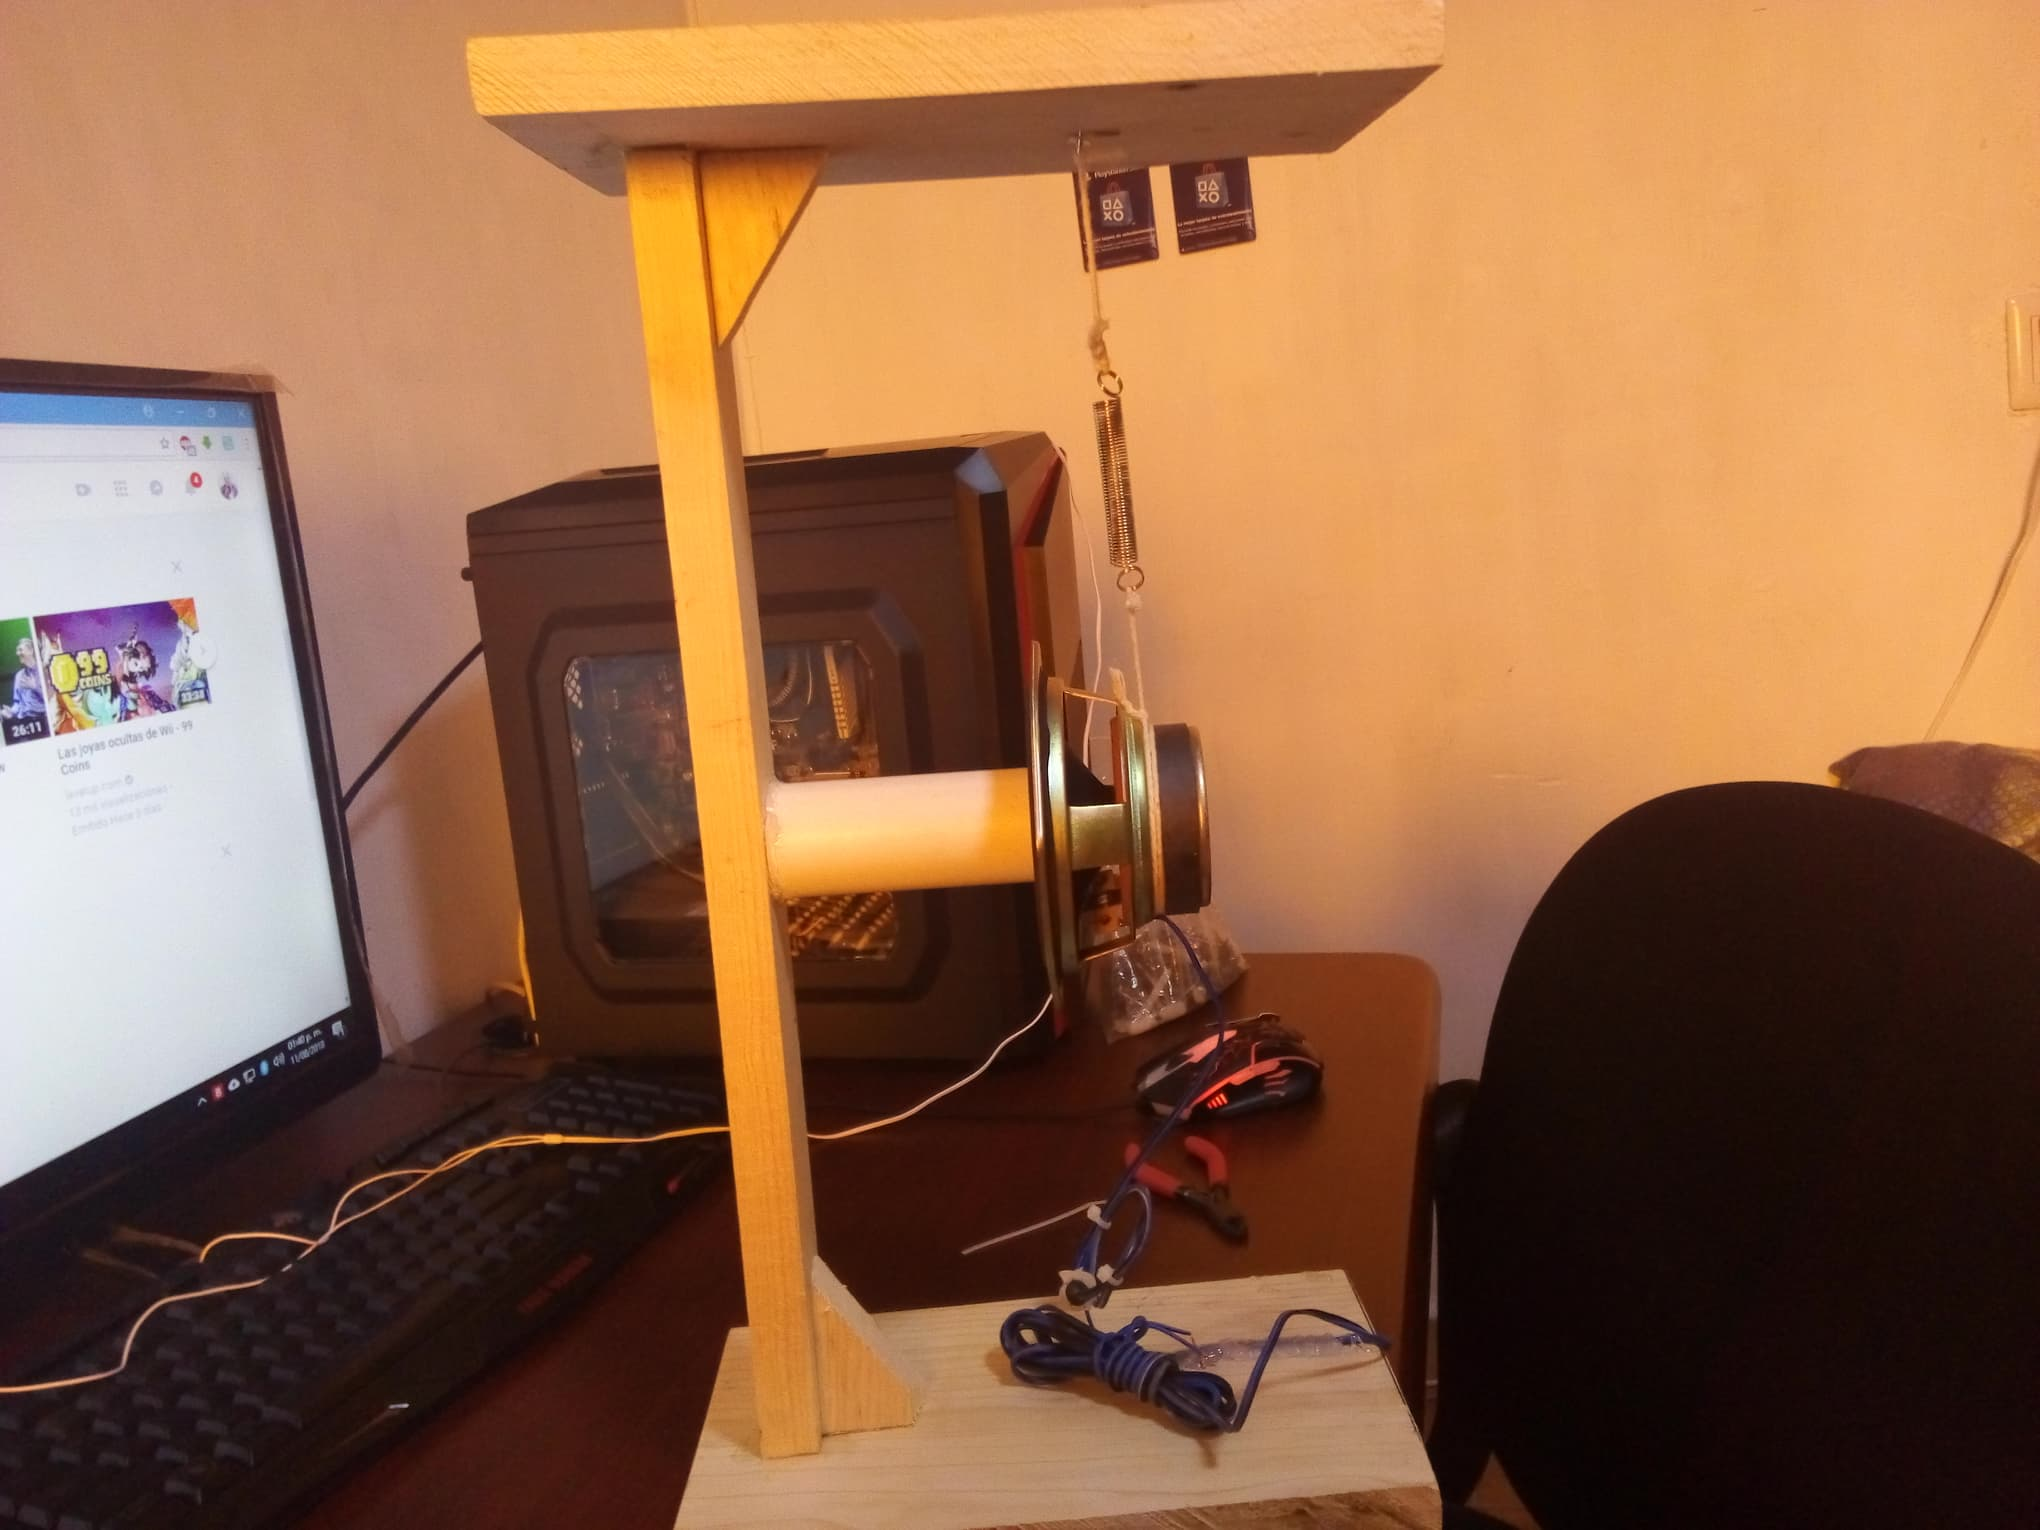
\includegraphics[width=0.5\textwidth]{Sismografo/Images/Inicial.png}
            \end{wrapfigure}
            
            Después de haber conseguido los materiales, se unieron como se puede ver en la imagen, observando que se ensamblo de modo que soporte el movimiento de forma correcta.
	        
            Se procuro que el tubo PVC quedara de forma horizontal sosteniendo a la bocina, haciendo que se mantuviera rígida. También se dejaron dos cables que salieran de la bocina de manera que fuera posible medir las señales que se generan. El resorte quedo sosteniendo la bocina a la base de madera, lo cual permite obtener la señal que se genera del movimiento.

             \subsubsection{Funcionamiento}
	        Cuando se tiene un movimiento relativo entre la bocina y la base generan un voltaje eléctrico el cual posteriormente será analizado. Internamente nuestra bocina trabaja con un campo magnético que es producido por el imán que contiene.

  \begin{figure}[htbp]
  \subsubsection{Sensor sísmico: Geófono armado}
\centering
\subfigure{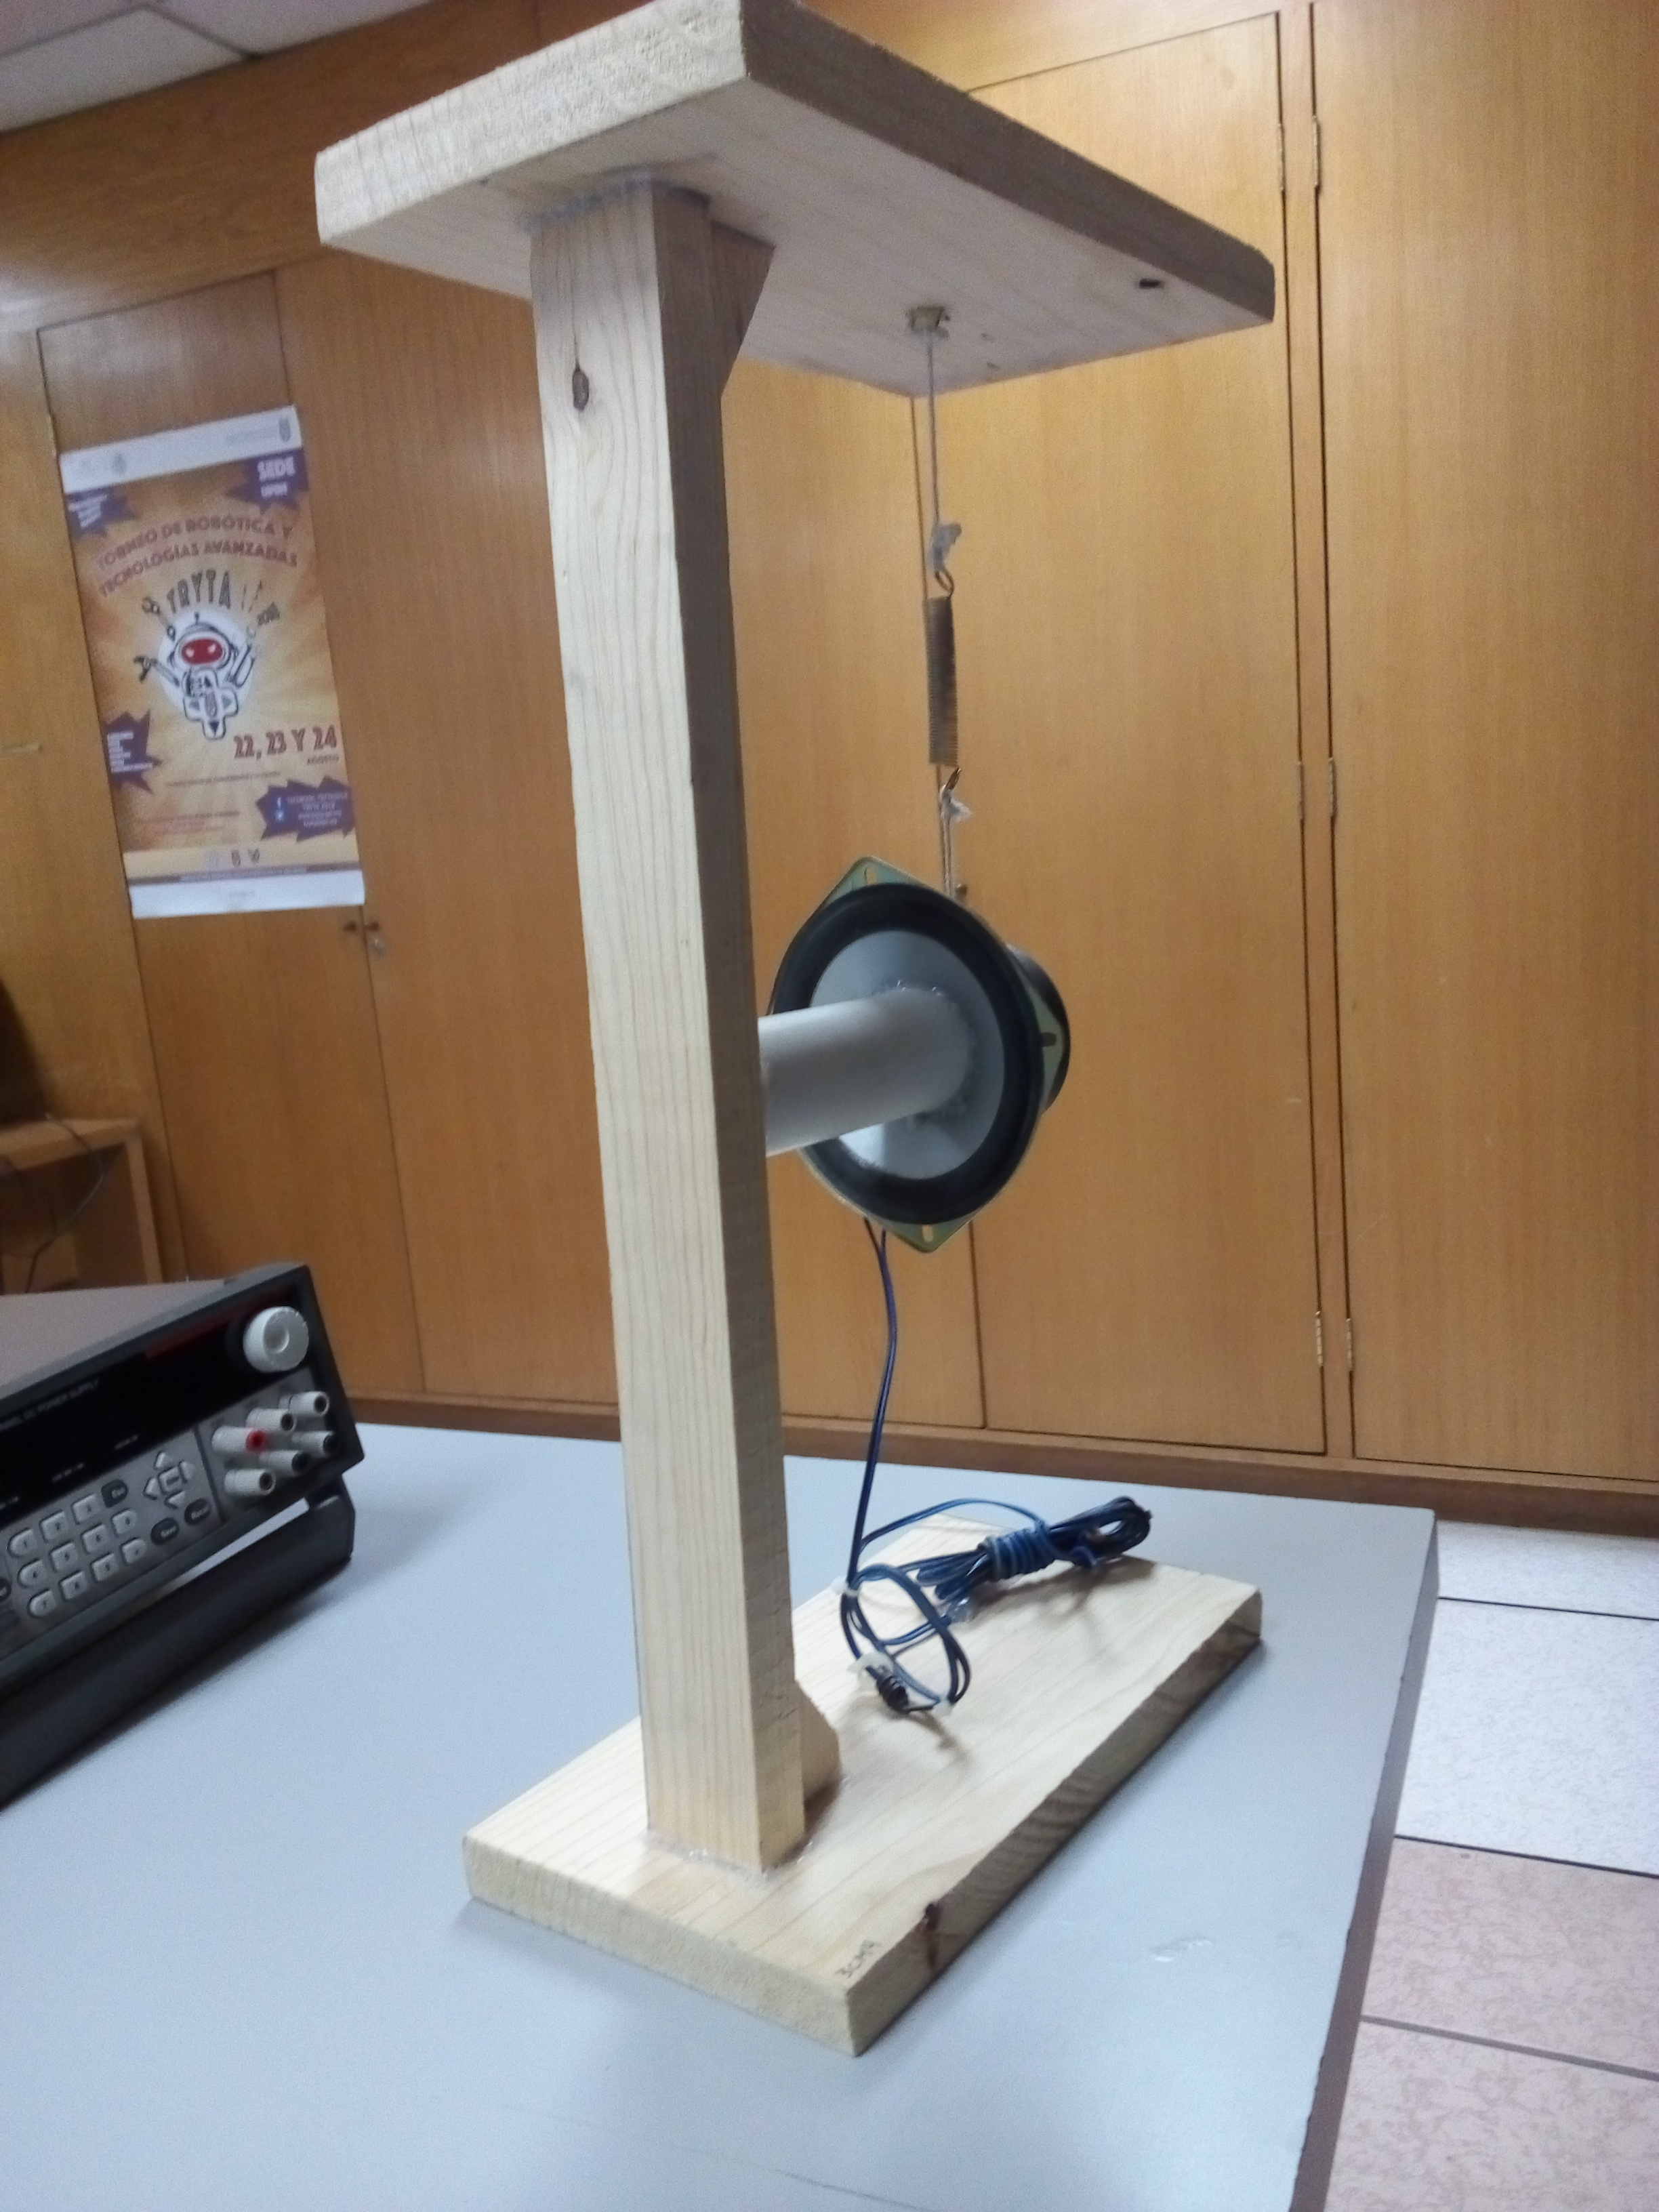
\includegraphics[width=0.45\textwidth]{Sismografo/Images/geo1.jpg}}
\subfigure{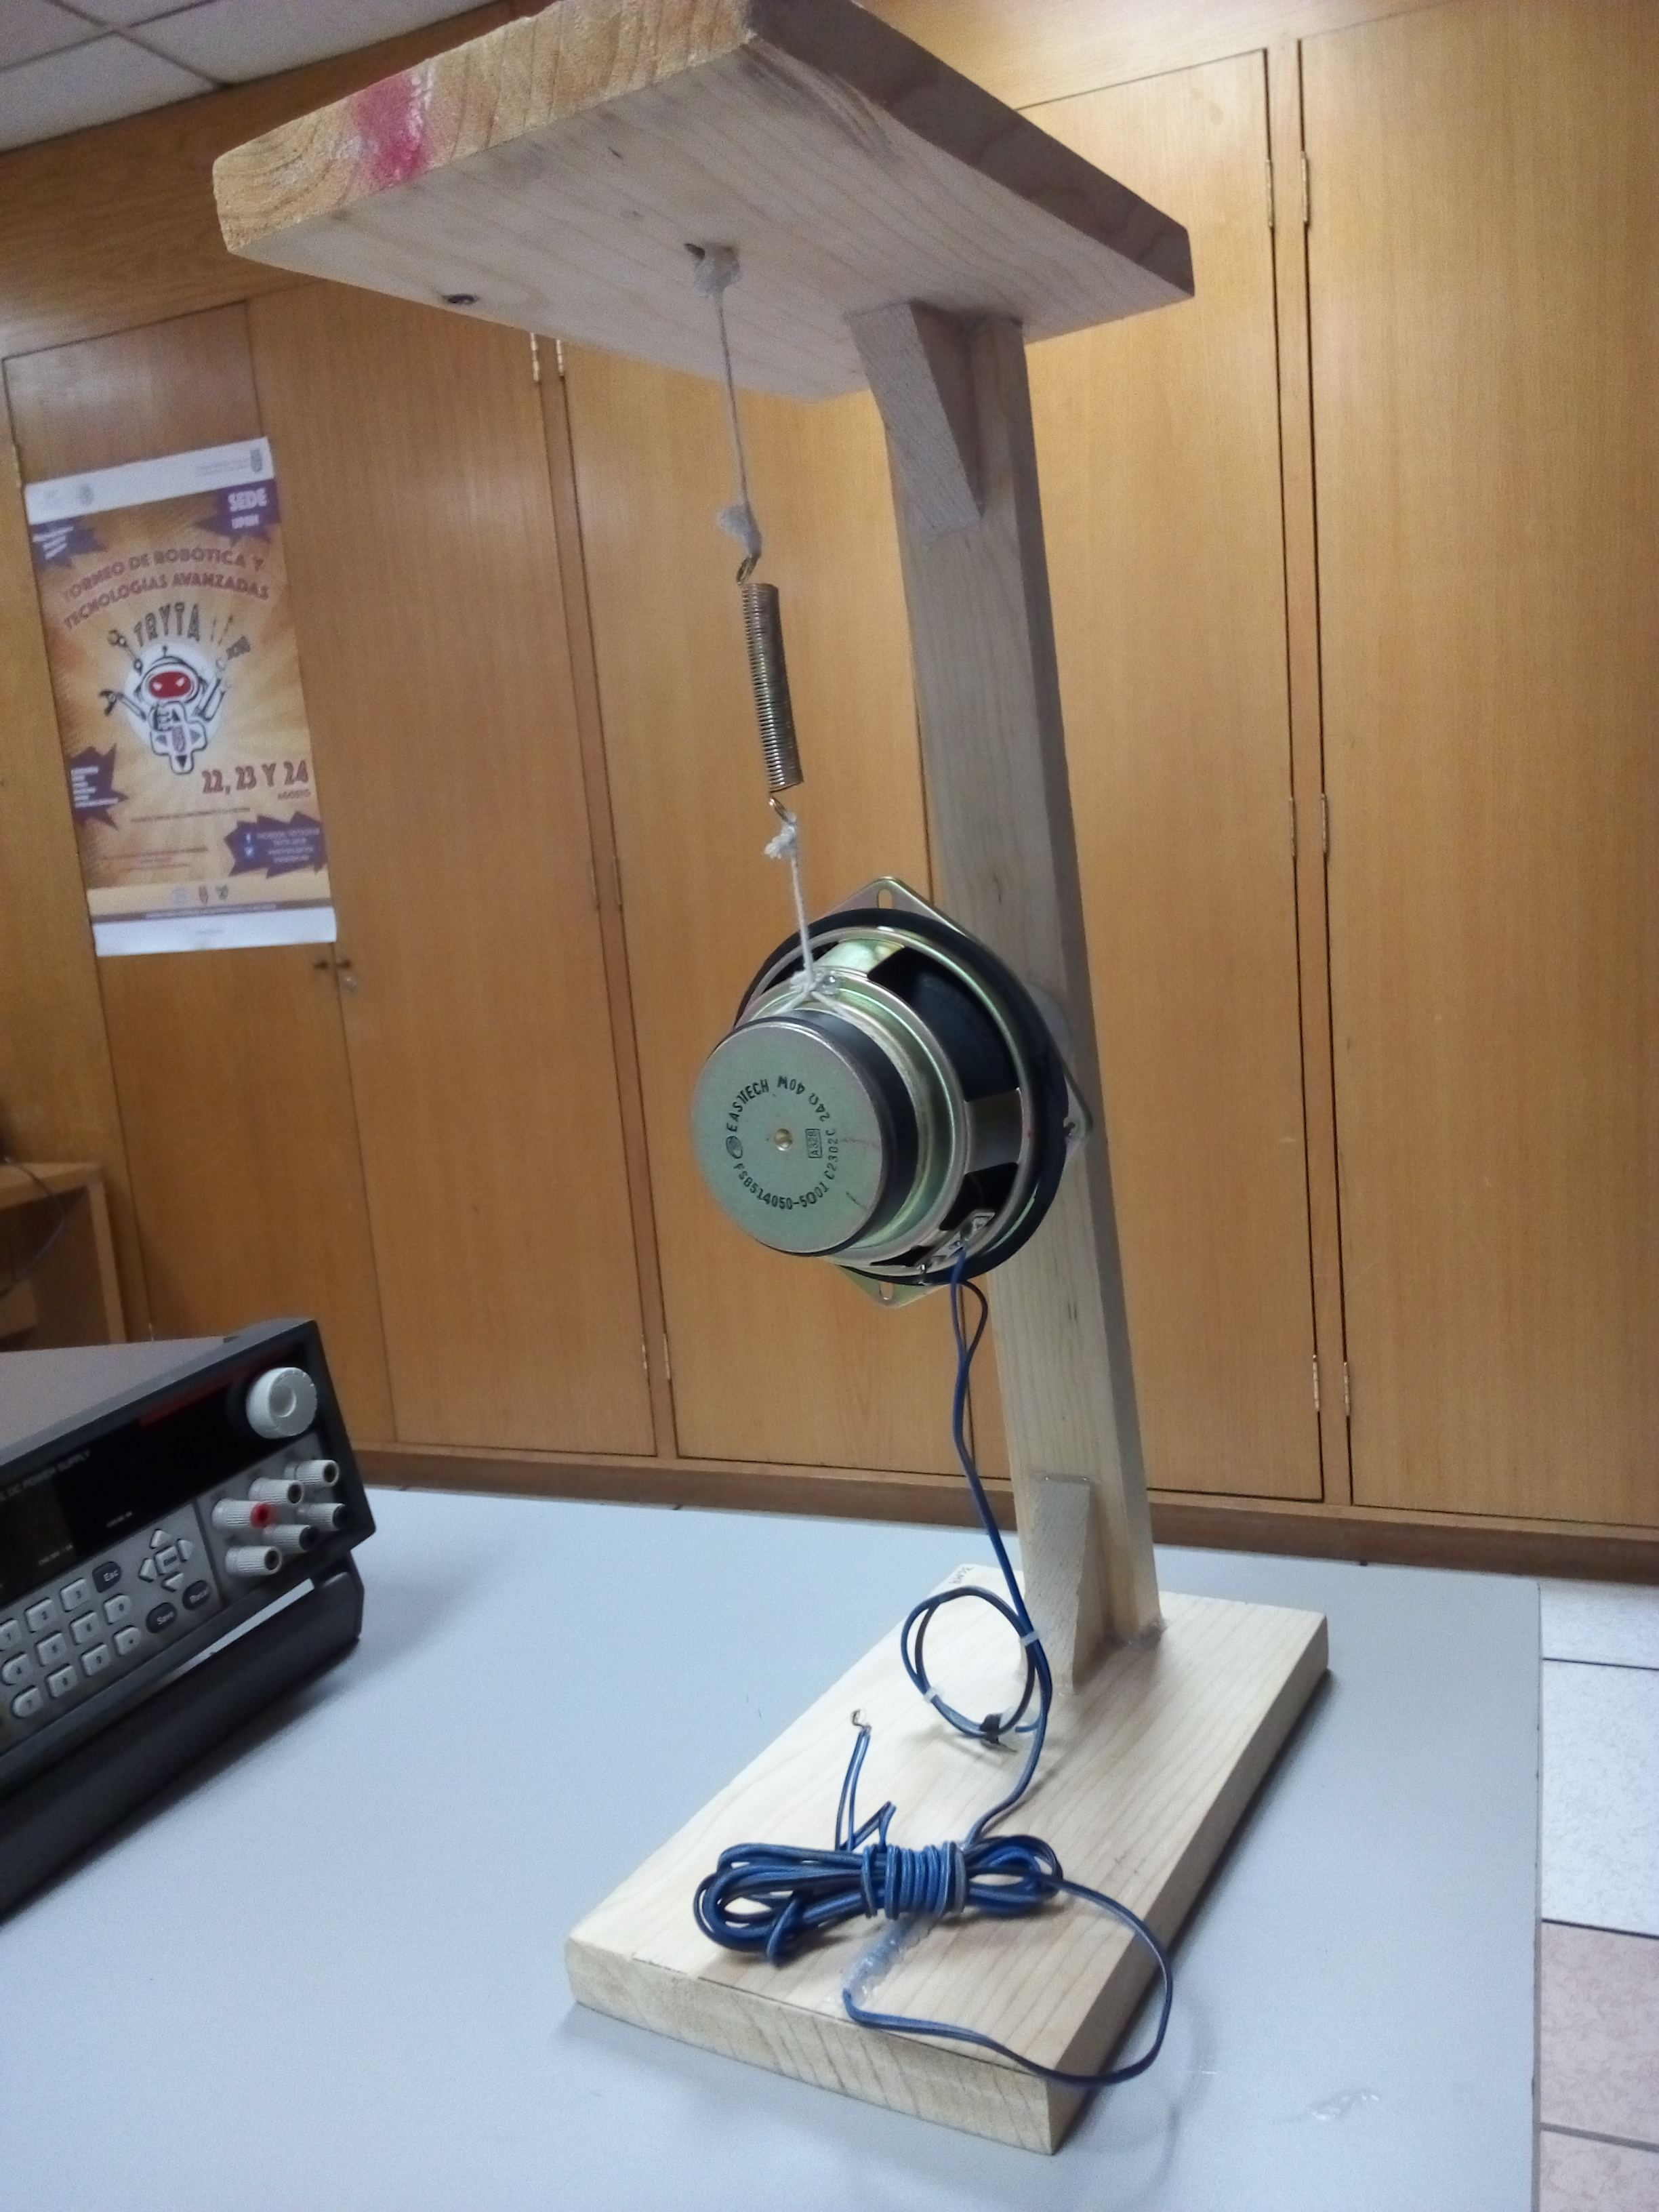
\includegraphics[width=0.45\textwidth]{Sismografo/Images/geo4.jpg}}
\subfigure{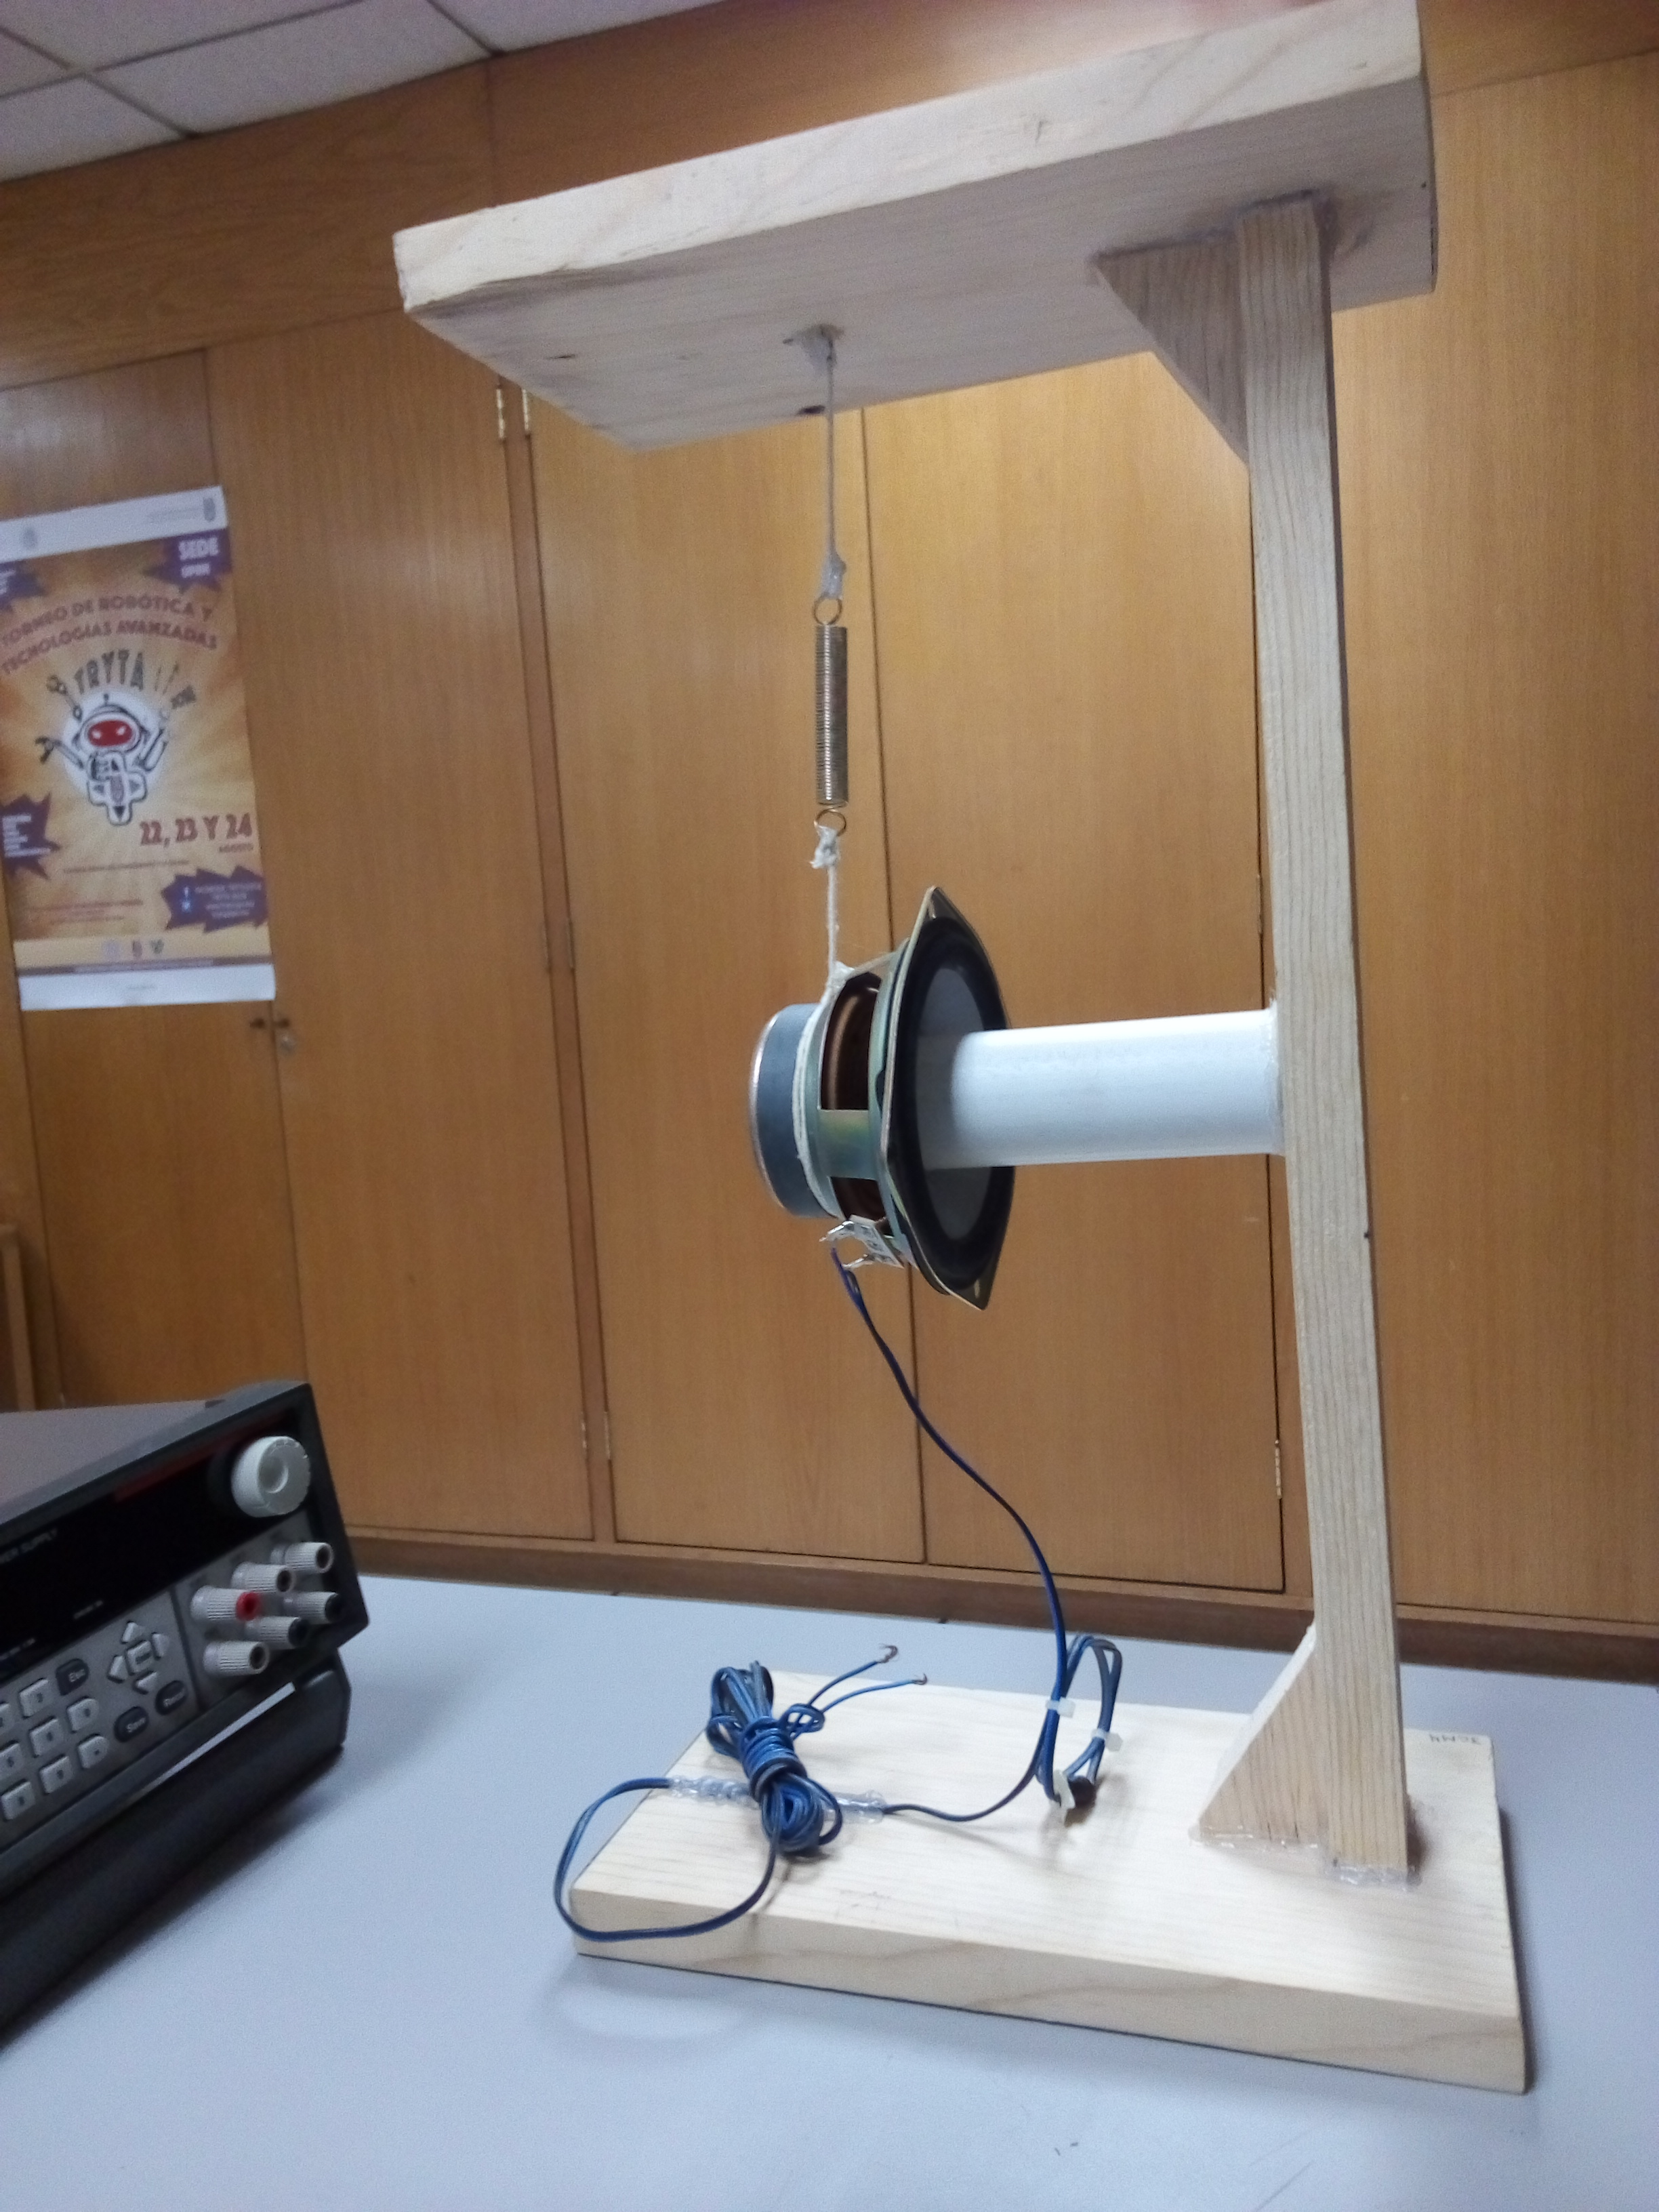
\includegraphics[width=0.45\textwidth]{Sismografo/Images/geo5.jpg}}
\subfigure{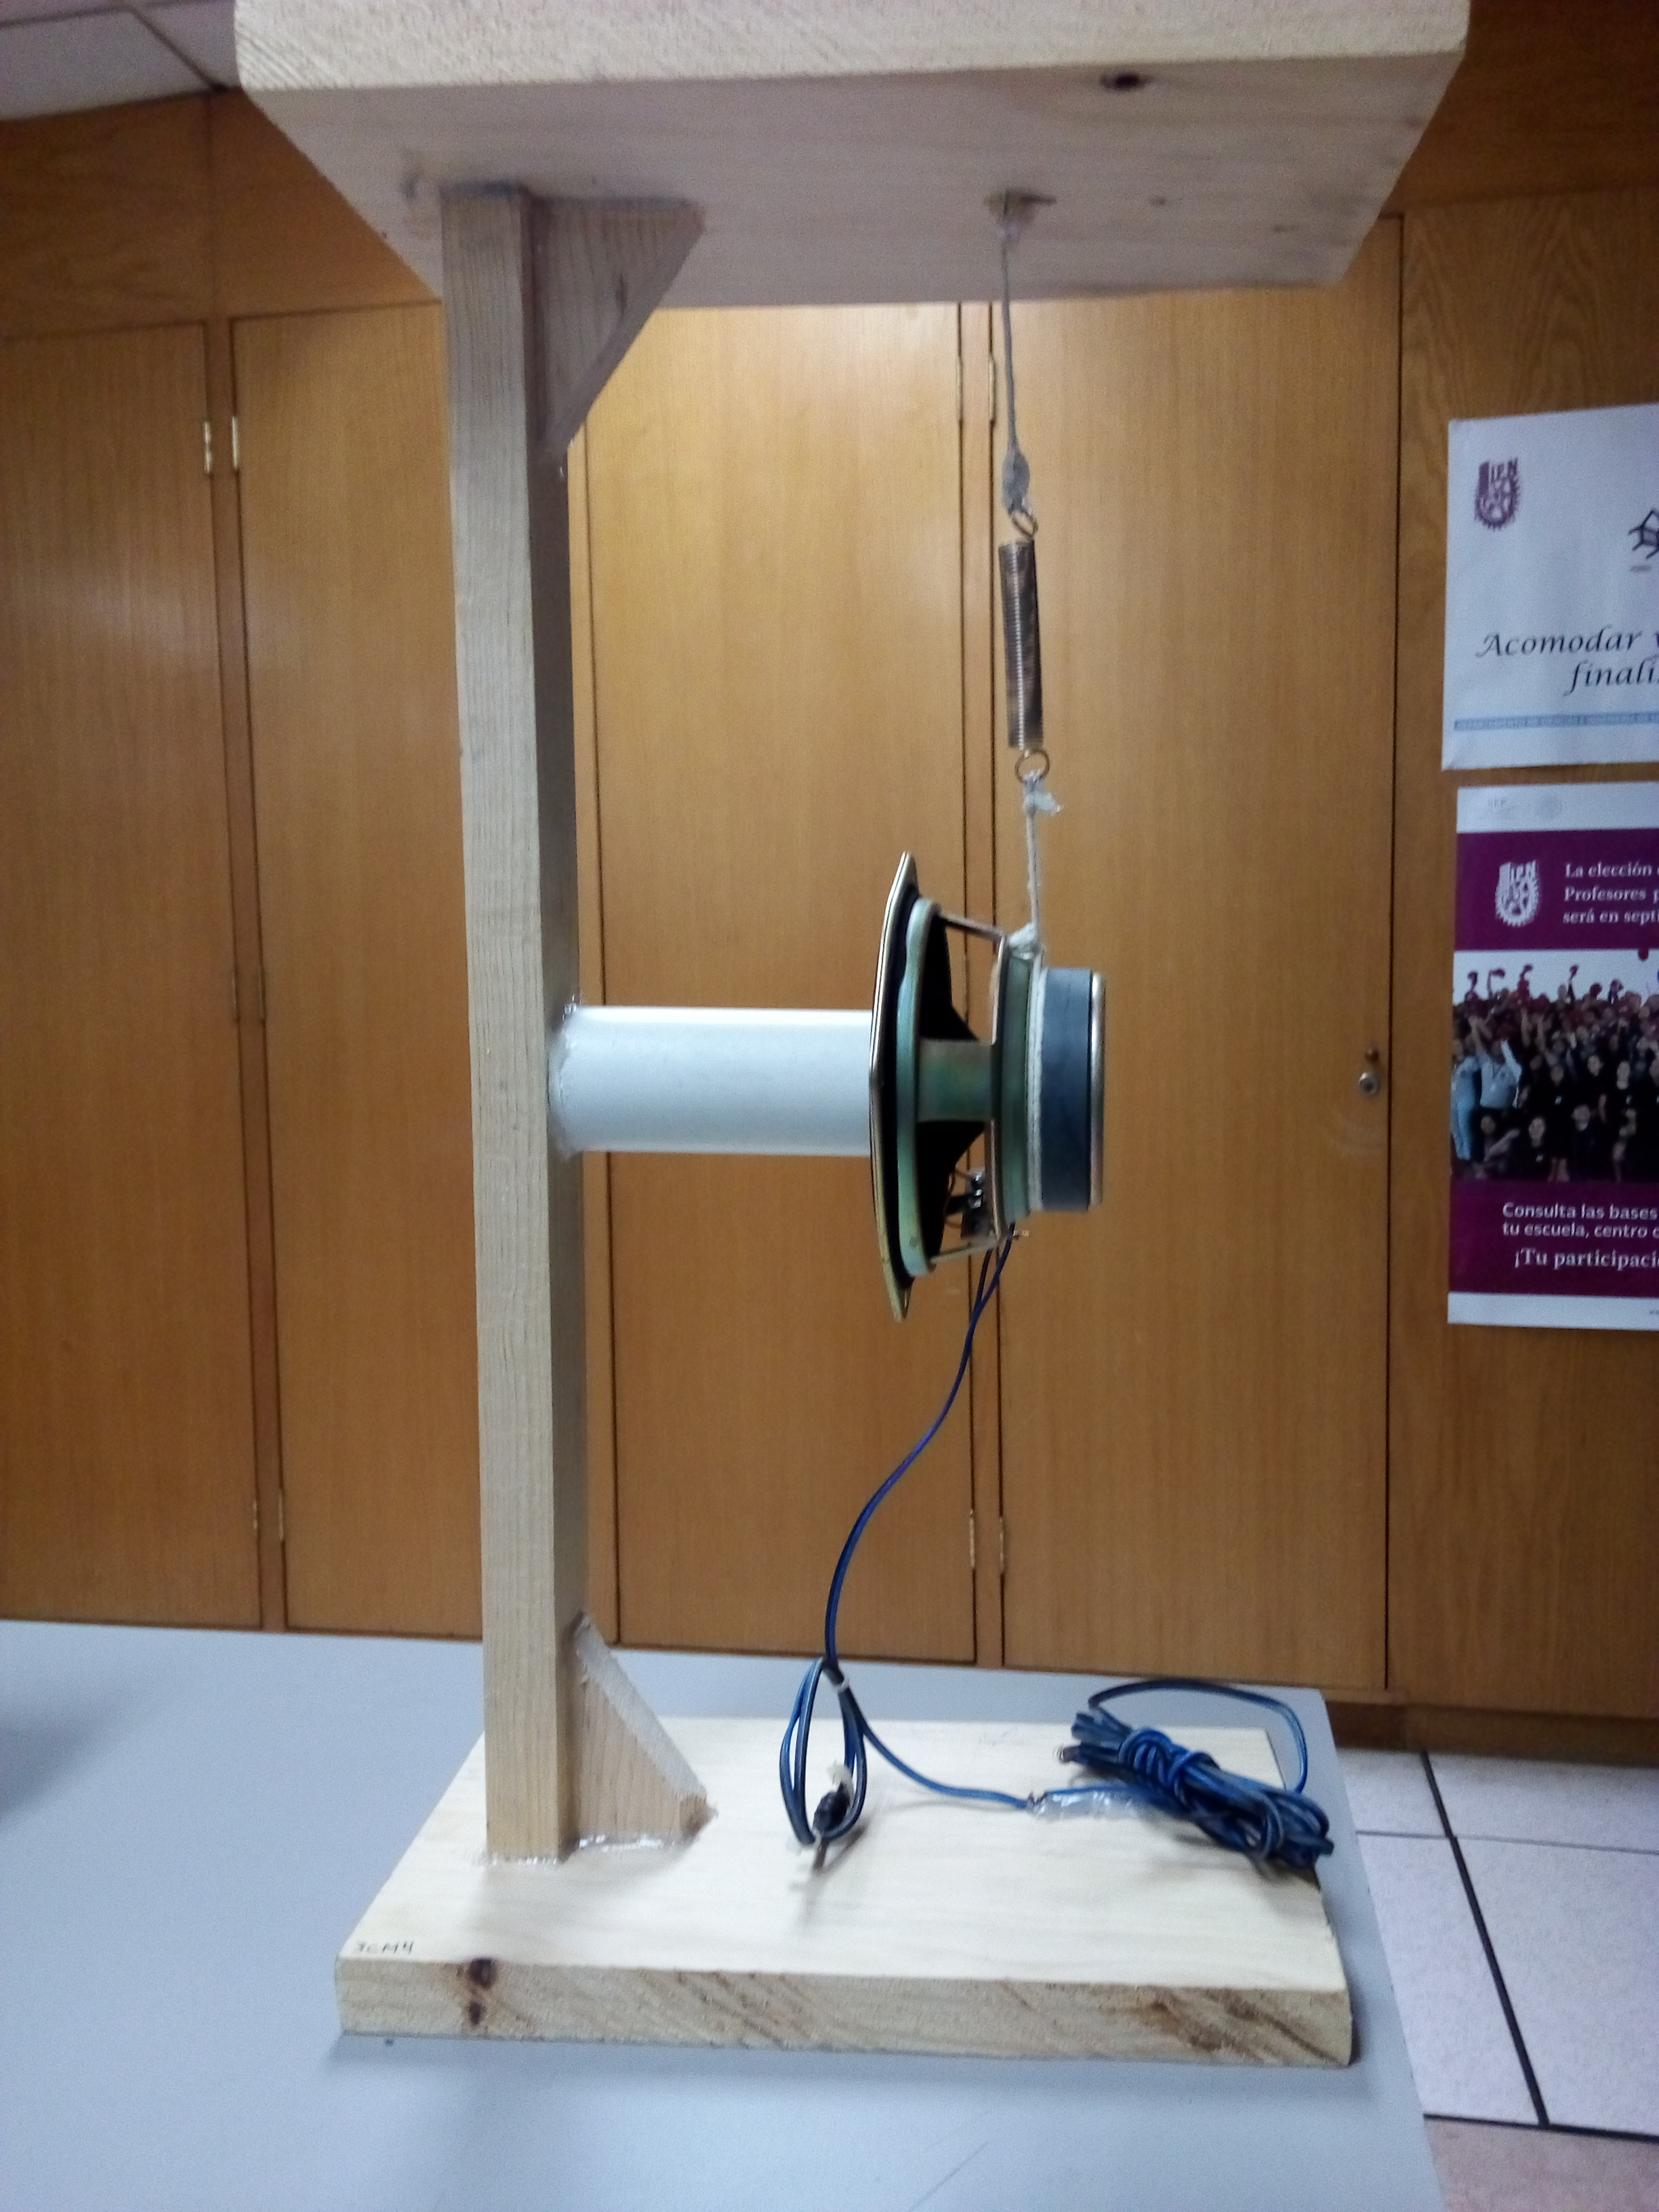
\includegraphics[width=0.45\textwidth]{Sismografo/Images/geo7.jpg}}

\end{figure}
            
	        \newpage
	       
	        
	        \subsubsection{Esquema de conexión para la primera medición}
	        Como se menciono, se dejo un cable para poder ver las señales, con ayuda de un cable BNC-caimán, lo conectamos a el canal 2 (puede ser al canal que se desee) del osciloscopio y ajustamos como en la siguiente sección se mostrara.
	        
    	        \begin{figure}[H]
        	       \centering
        	       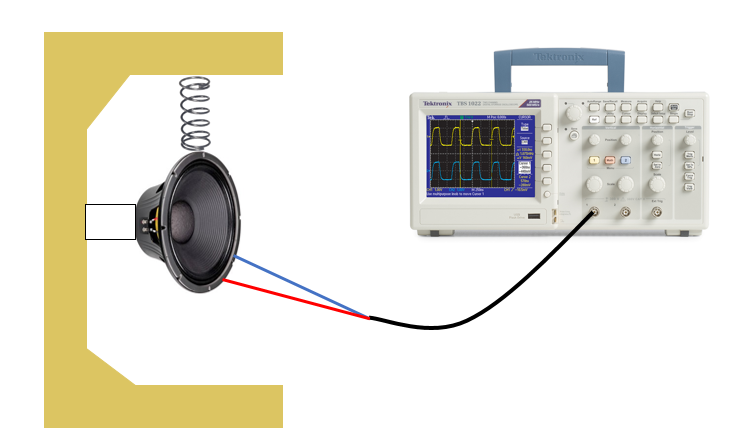
\includegraphics[scale=0.55]{Images/EsquemaConexion.PNG}
        	    \end{figure}
	        
	        \subsubsection{Medición de amplitud de señal - voltaje}
	        % AQUÍ VA -	Mida la oscilación máxima con el osciloscopio (Valor Vpp) e indíquela con unidades, respaldar la medición con la captura de pantalla e indique los parámetros de ajuste del osciloscopio (base de tiempo, volts por división, acoplamiento de señal), recuerde que la medición es simulando el movimiento con el cajón de prueba
	        
            \textbf{Parámetros de medición (Vpp)}
            \begin{multicols}{2}
                \begin{itemize}
                    \item[\checkmark] \textbf{Amplitud máxima: 880 mV}
                    \item[\checkmark] \textbf{Base de tiempo: 250 ms}
            \columnbreak
                    \item[\checkmark] \textbf{Volts por división: 200 mV}
                    \item[\checkmark] \textbf{Acoplamiento: Corriente Continua}
                \end{itemize}
            \end{multicols}
            
	        % PONER FOTO DE LA MEDICIÓN PURA, ES DECIR DIRECTAMENTE AL OSCILOSCOPIO
	        \begin{figure}[h!]
                \centering
                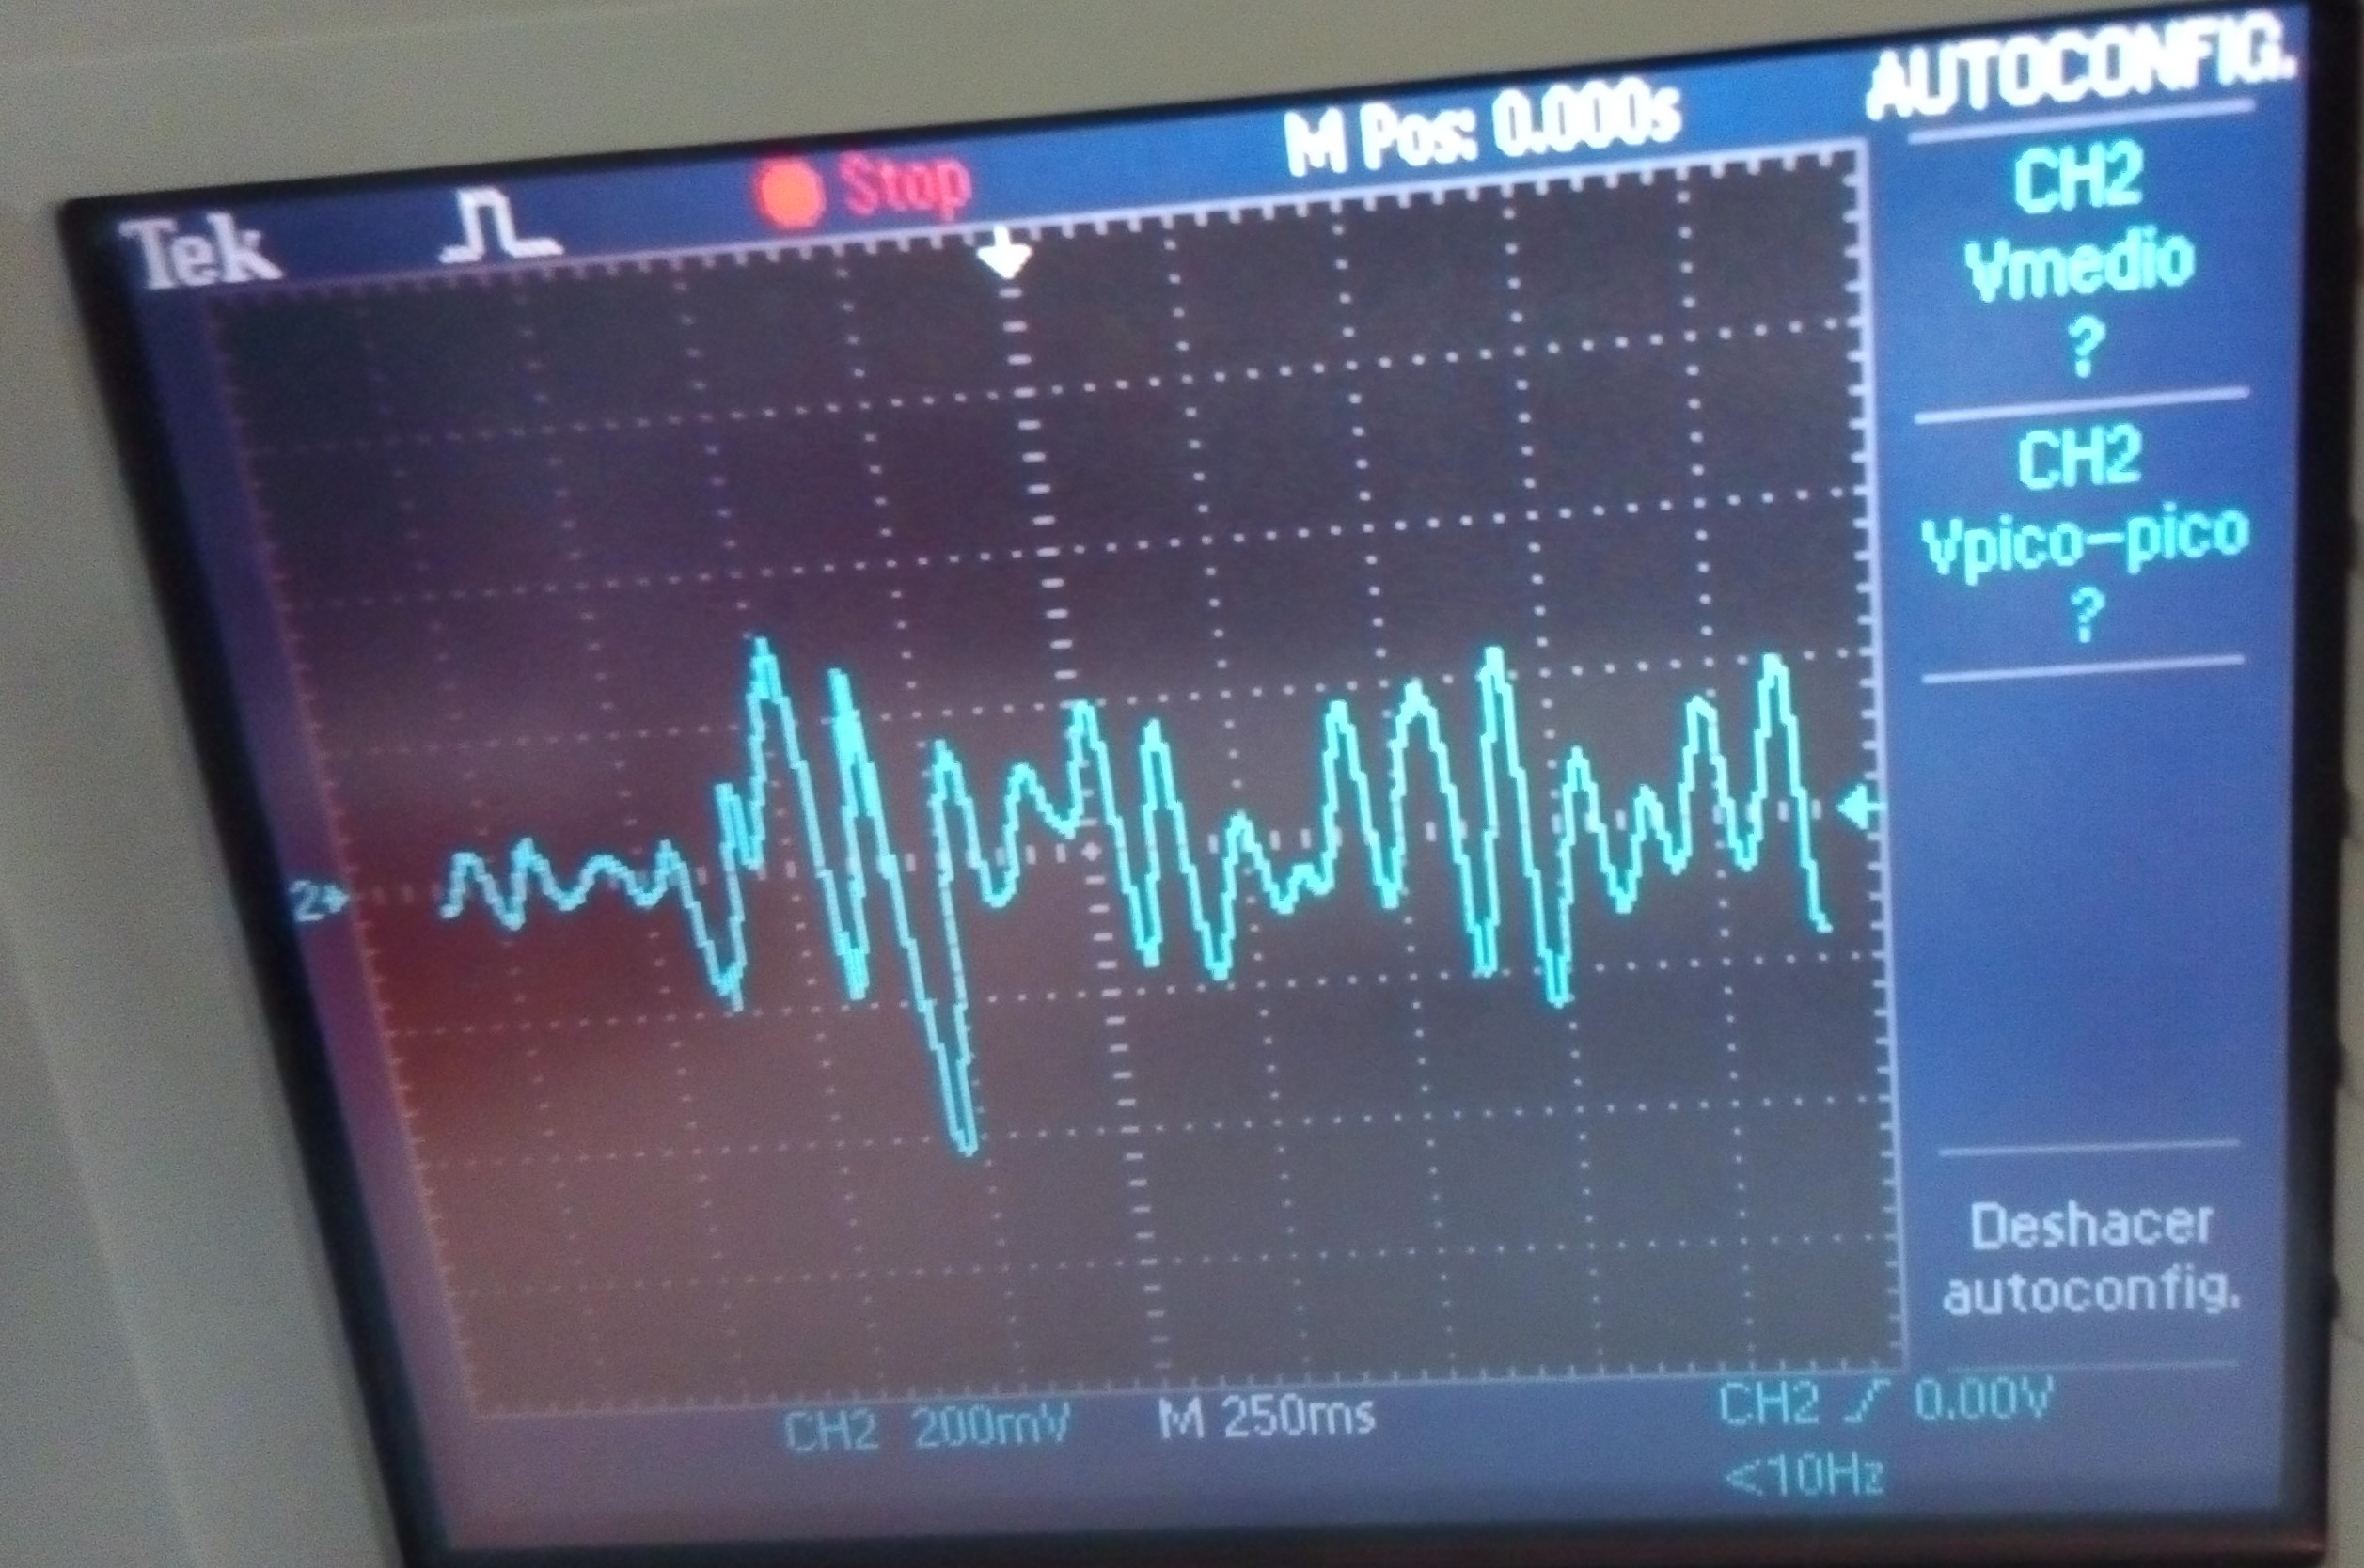
\includegraphics[width=0.7\textwidth]{Sismografo/Images/PE1_1.jpg}
            \end{figure} 
	        \newpage
	    %/////////////////////////////////////////////////////////////////
    	%                   PROCEDIMIENTO EXPERIMENTAL 2
    	%/////////////////////////////////////////////////////////////////	    
	    \subsection{PE 2 - Filtrado de señal}
	        \subsubsection{Rangos de frecuencia}
	        % -	De acuerdo a la teoría sísmica investigada elija el rango de frecuencias adecuado para realizar la medición de sismos, explique porque es la adecuada, esta será la frecuencia de corte para el filtro a diseñar.
	        Según la teoría sísmica investigada, el rango de frecuencias adecuado para realizar la medición de sismos fue \textbf{1 - 100 Hz}, sin embargo, fuentes de información mencionan que no llega a pasar de 10 Hz, por lo cual los cálculos se realizaron con la frecuencia de \textbf{12 Hz}.
	        
	        \subsubsection{Filtro}
	        % -	Indicar de que tipo es su filtro, de que orden, realice los cálculos necesarios  y haga un esquema de circuito indicando sus valores y los puntos de medición. Si tiene integrado una primera etapa amplificadora esta deberá ser ajustada a una ganancia igual a 10.
	        \textbf{Datos generales}
	        \begin{itemize}
	            \item Tipo de filtro: Pasa bajas
	            \item Orden de filtro: Segundo orden
	        \end{itemize}
	        
	        
	        \textbf{Esquema de circuito}
	        % PONER ESQUEMA DEL CIRCUITO FILTRO PASABAJAS
	        El esquema del filtro pasa bajas, que consta de un LM741 con 2 valores de resistencias y capacitores, es el siguiente:
	       
	        \begin{figure}[h!]
                \centering
                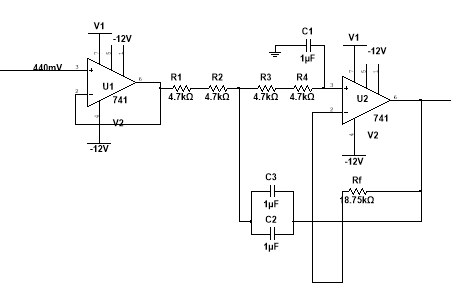
\includegraphics[width=0.7\textwidth]{Sismografo/Images/E_FILTRO.PNG}
            \end{figure} 
            
            Como se aprecia en el circuito, se colocaron arreglos de resistencias en serie y capacitores en paralelo debido a que los valores obtenidos no existen de forma comercial.
	        
	        Sin embargo en nuestro circuito previamente también tenemos un buffer de entrada utilizando otro LM741 como seguidor de voltaje, que adapta el nivel de salida de alta impedancia de geófono, al filtro con un nivel de entrada de baja impedancia. 
	        \newpage
	        El esquema es el siguiente:
	        
	        \begin{figure}[h!]
                \centering
                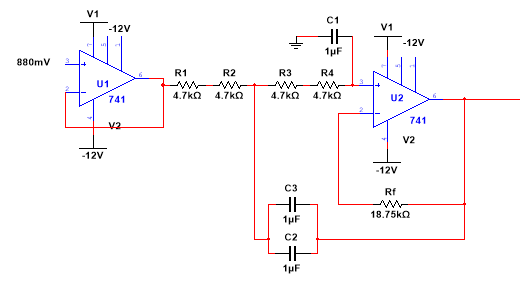
\includegraphics[width=0.8\textwidth]{Sismografo/Images/E_FILTROBUFFER.PNG}
            \end{figure} 
            
            \subsubsection{Circuito cableado:}
            \begin{figure}[h!]
                \centering
                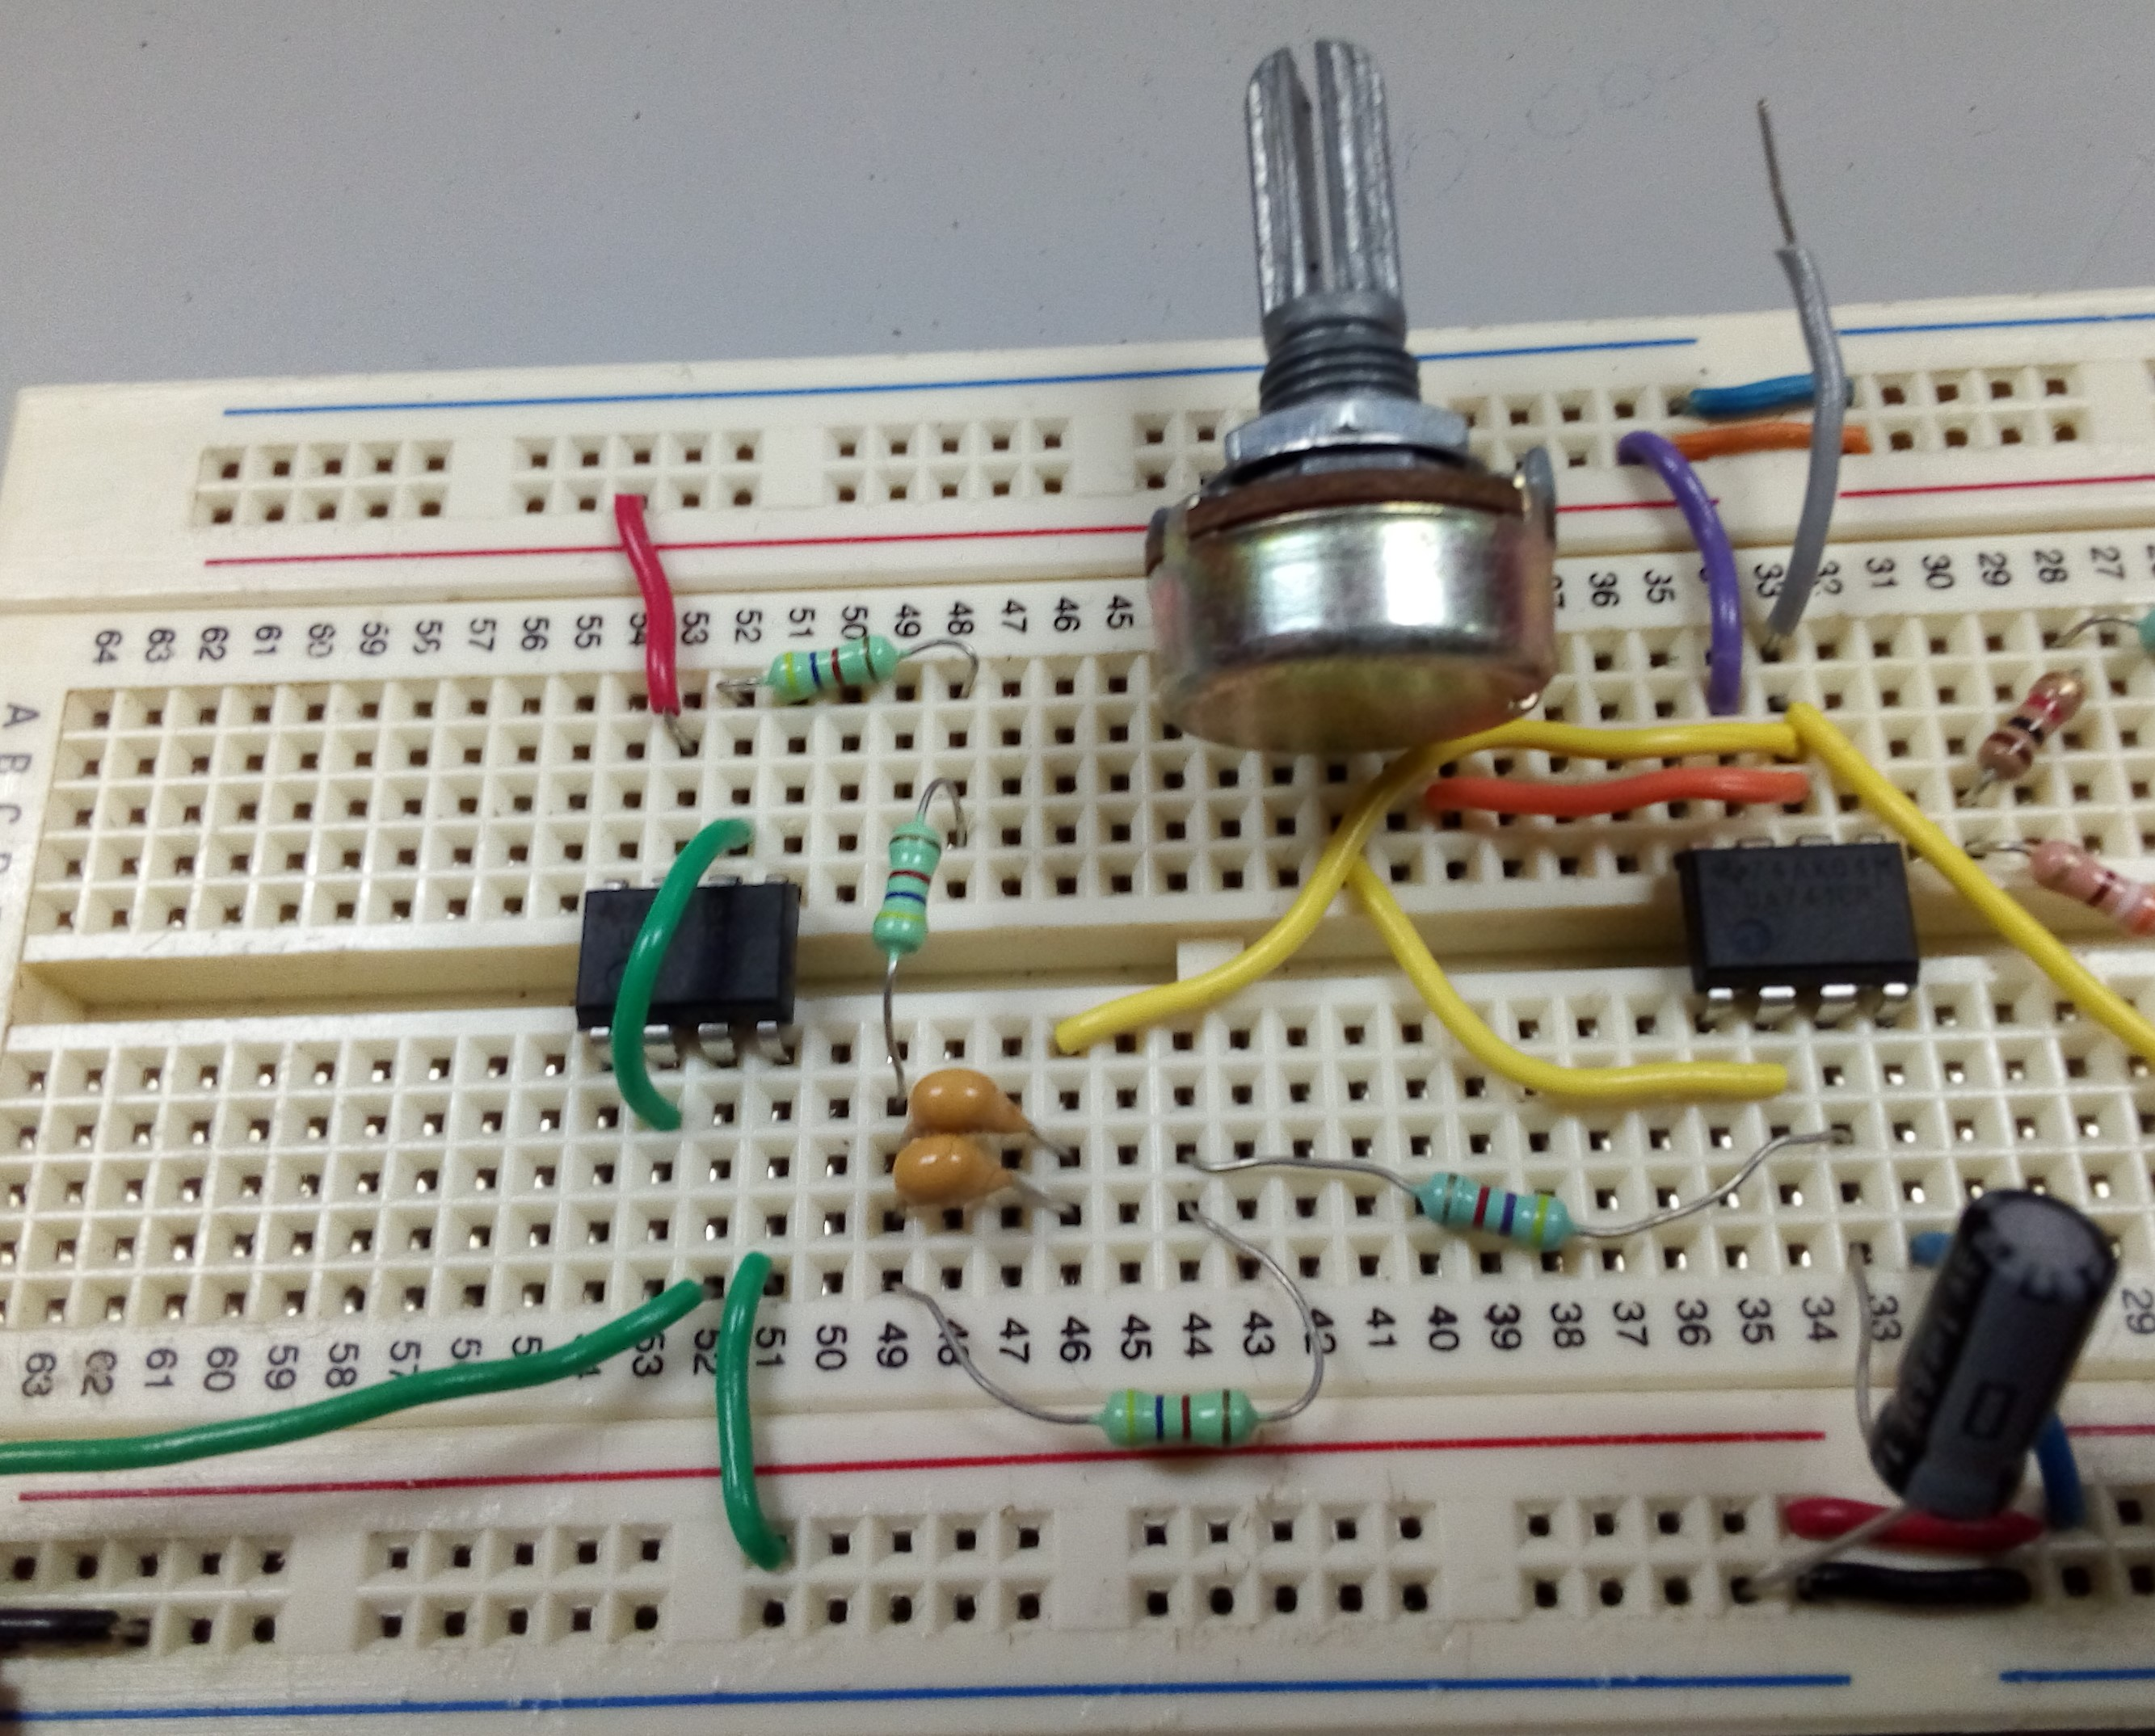
\includegraphics[width=0.8\textwidth]{Sismografo/Images/cfiltro1.jpg}
            \end{figure}


	        \subsubsection{Medición de amplitud de señal - voltaje}
	        % -	Mida la oscilación máxima con el osciloscopio (Valor Vpp) a la salida del circuito de filtro e indíquela con unidades, respaldar la medición con la captura de pantalla e indique los parámetros de ajuste del osciloscopio (base de tiempo, volts por división, acoplamiento de 
	       
	        \textbf{Parámetros de medición (Vpp)}
            \begin{multicols}{2}
                \begin{itemize}
                    \item[\checkmark] \textbf{Amplitud máxima entrada: 880 mV}
                    
                    \item[\checkmark] \textbf{Base de tiempo: 250 ms}
            \columnbreak
                    \item[\checkmark] \textbf{Volts por división: 200 mV}
                    \item[\checkmark] \textbf{Acoplamiento: Corriente Continua}
                \end{itemize}
            \end{multicols}
            
            \textbf{Nota:} La linea azul es la señal del filtro y la amarilla la que sale directamente de la bocina.
            
	        % PONER FOTO DE LA MEDICIÓN CON LA ETAPA DE FILTRADO
	        \begin{figure}[h!]
                \centering
                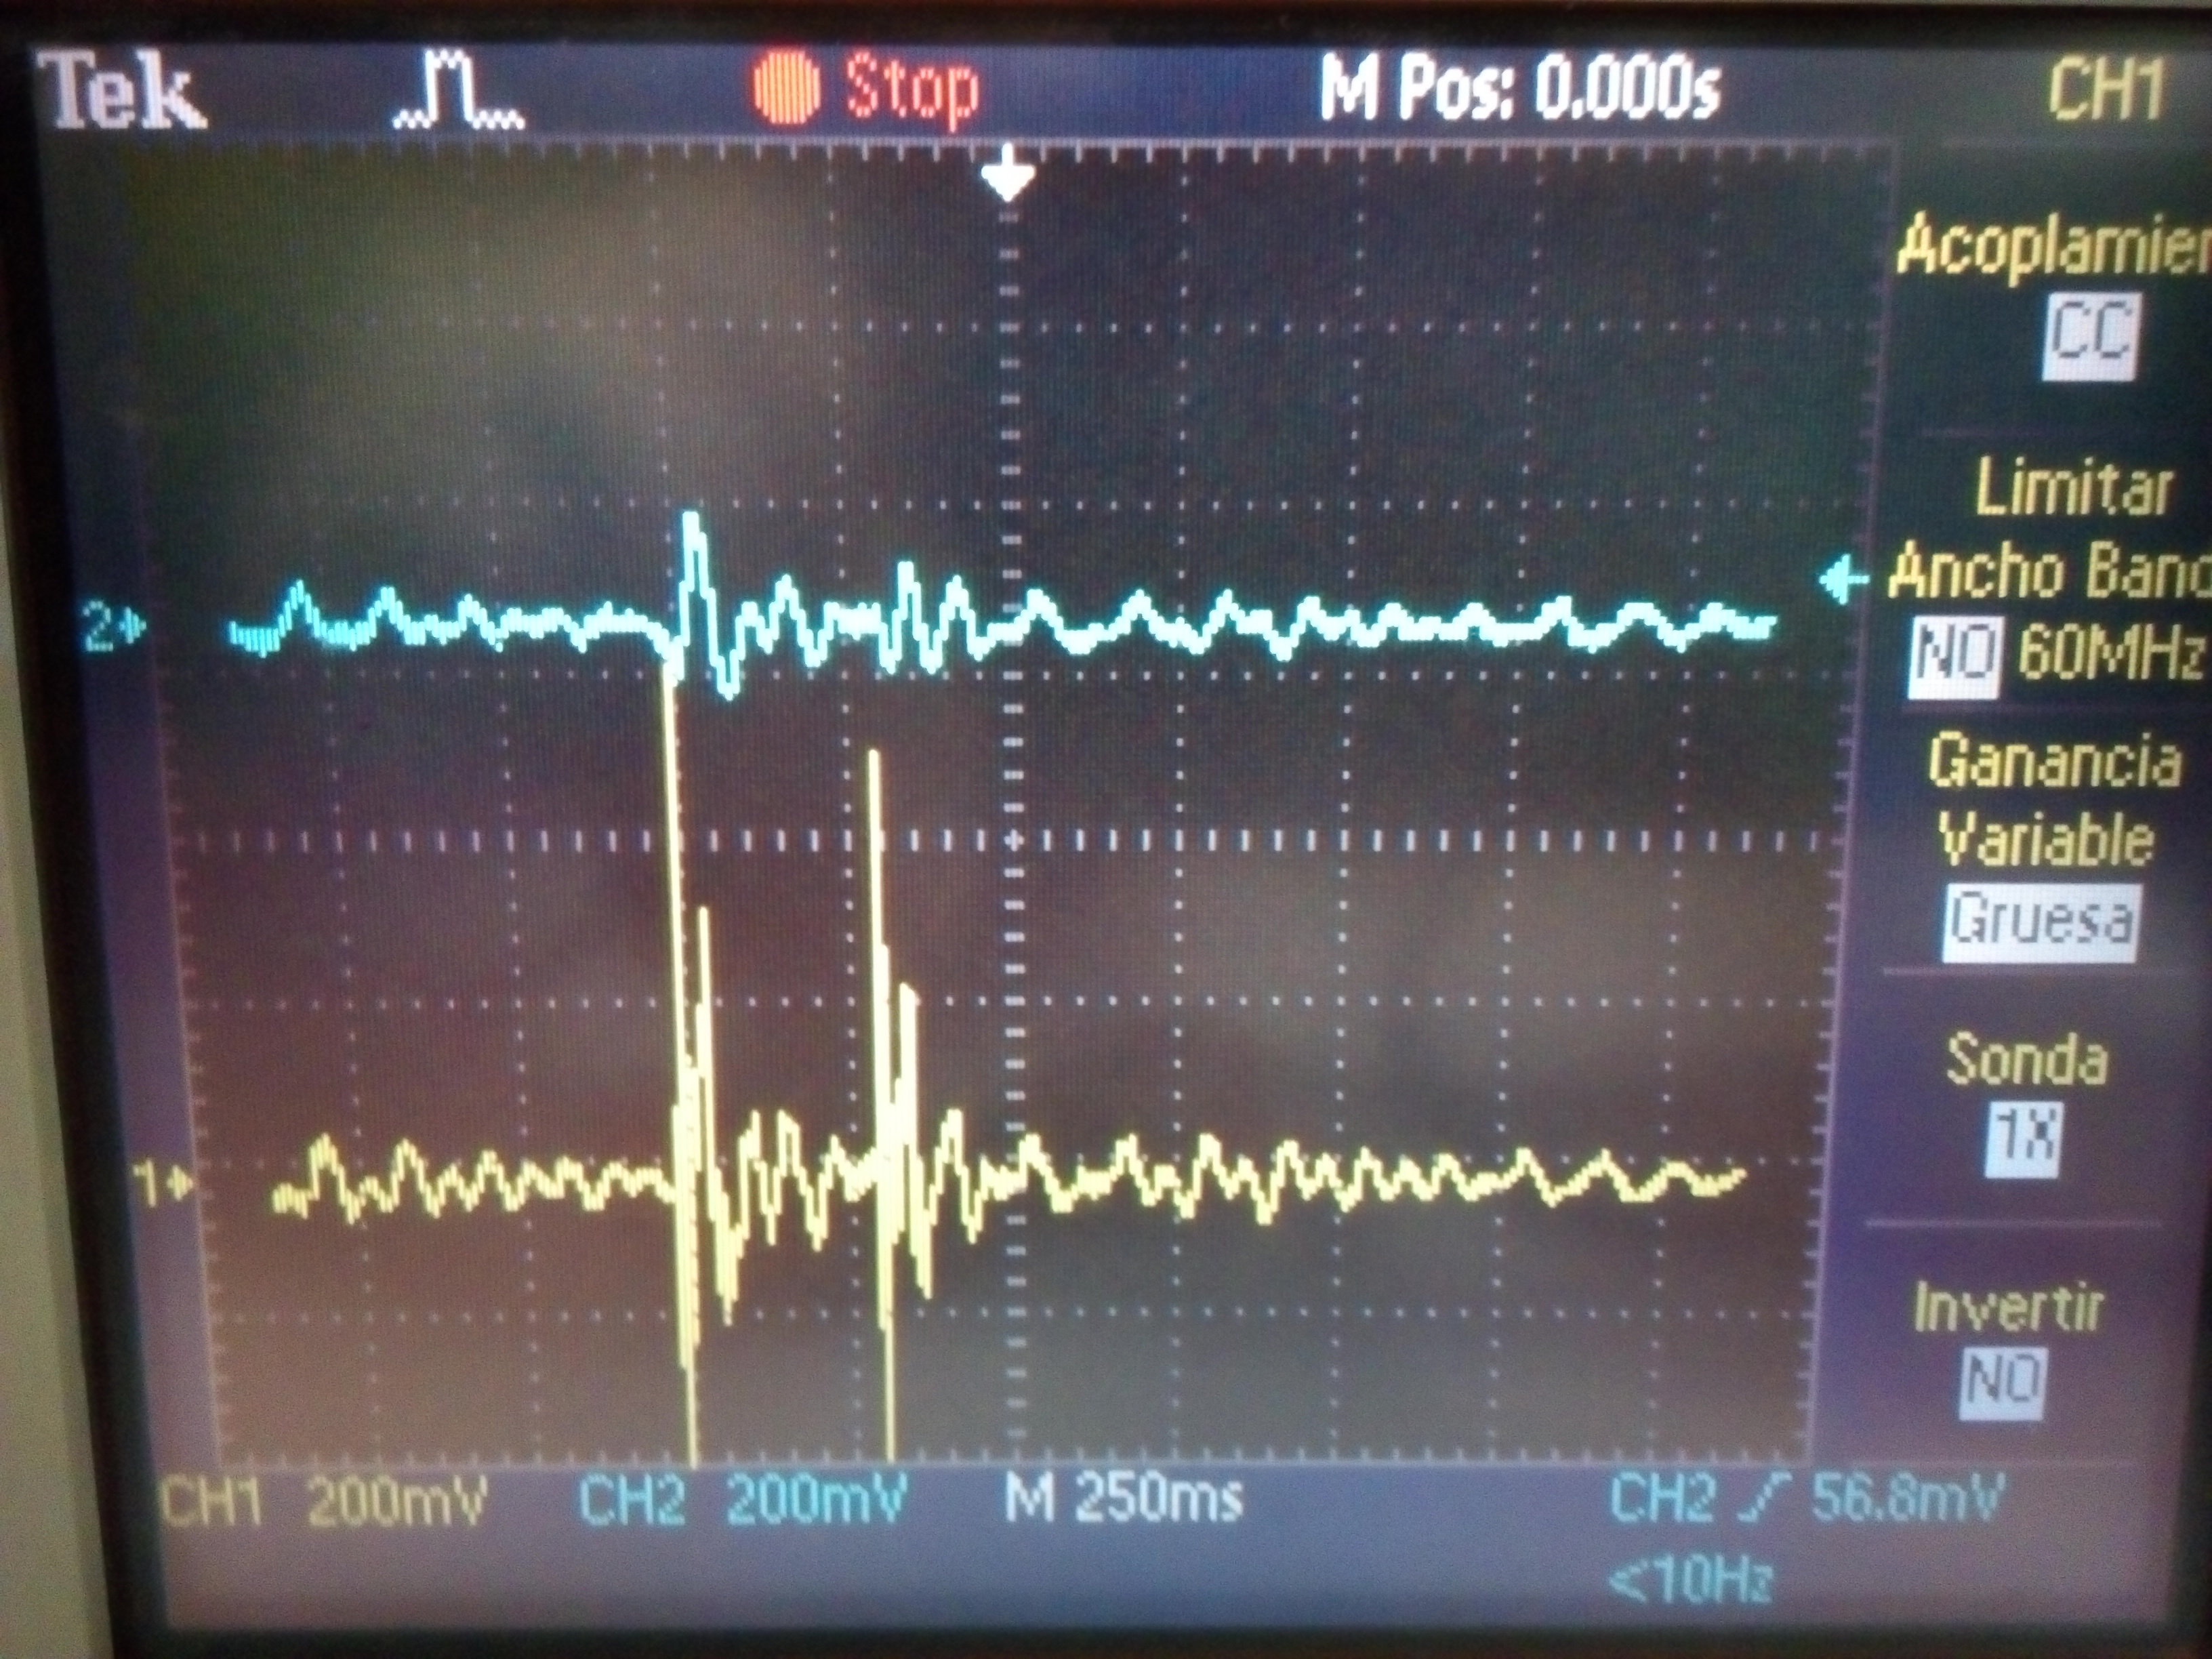
\includegraphics[width=0.7\textwidth]{Sismografo/Images/filtro.jpg}
            \end{figure} 

	        \subsubsection{Explicación del funcionamiento del filtro}
	        % -	Explique cómo comprobó el funcionamiento de su filtro.
	        El funcionamiento del filtro se comprobó al comparar la señal directamente de la entrada (amarillo en la imagen) y la señal de salida después del filtro (azul en la imagen), pudimos ver que era correcto puesto que el objetivo del filtro era que no se tomaran las señales generadas por pequeños golpes a la mesa, cuando pase un carro, entonces decidimos golpear la mesa y el filtro funciono correctamente como se ve en la parte de medición.
	        
	        De esta forma, eliminamos ruido en nuestra señal y evitamos que aquellas de origen distinto a un sismo (es decir, que posen una frecuencia por encima de 12 Hz) pasen a la siguiente etapa del sensor: la Segunda etapa de amplificación.
	
	    %/////////////////////////////////////////////////////////////////
    	%                   PROCEDIMIENTO EXPERIMENTAL 3
    	%////////////////////////////////////////////////////////////////  
        \newpage
	    \subsection{PE 3- Segunda etapa de amplificación}
	    
	    Una vez filtrada la señal, necesitamos amplificarla. Como se habrá notado, la amplitud (voltaje) máxima de la señal esta en el orden de los mili volts, con lo cual es muy difícil obtener mediciones precisas. 
	    
	    Con ayuda de un amplificador no inversor 741, podremos aumentar nuestra señal hasta los 10Vpp, al orden de los volts en donde es más sencillo y práctico medir.
	    
	    \textbf{Datos generales}
	        \begin{itemize}
	            \item Tipo de amplificador: No inversor
	            \item Ganancia: 11.66
	        \end{itemize}

	        \subsubsection{Esquema de circuito}
	        
	        % PONER ESQUEMA DEL CIRCUITO AMPLIFICACIÓN
	        \begin{figure}[h!]
                \centering
                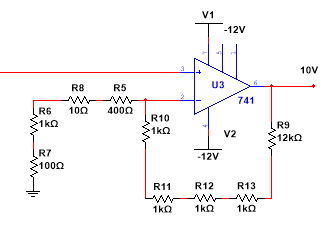
\includegraphics[width=0.7\textwidth]{Sismografo/Images/Amplificador.PNG}
            \end{figure} 
            
            Similar al diseño del filtro, se colocaron arreglos de resistencias en serie debido a que no poseíamos estos valores de resistencia al momento de armar el circuito.
            \newpage
            \subsubsection{Circuito cableado:}
            \begin{figure}[h!]
                \centering
                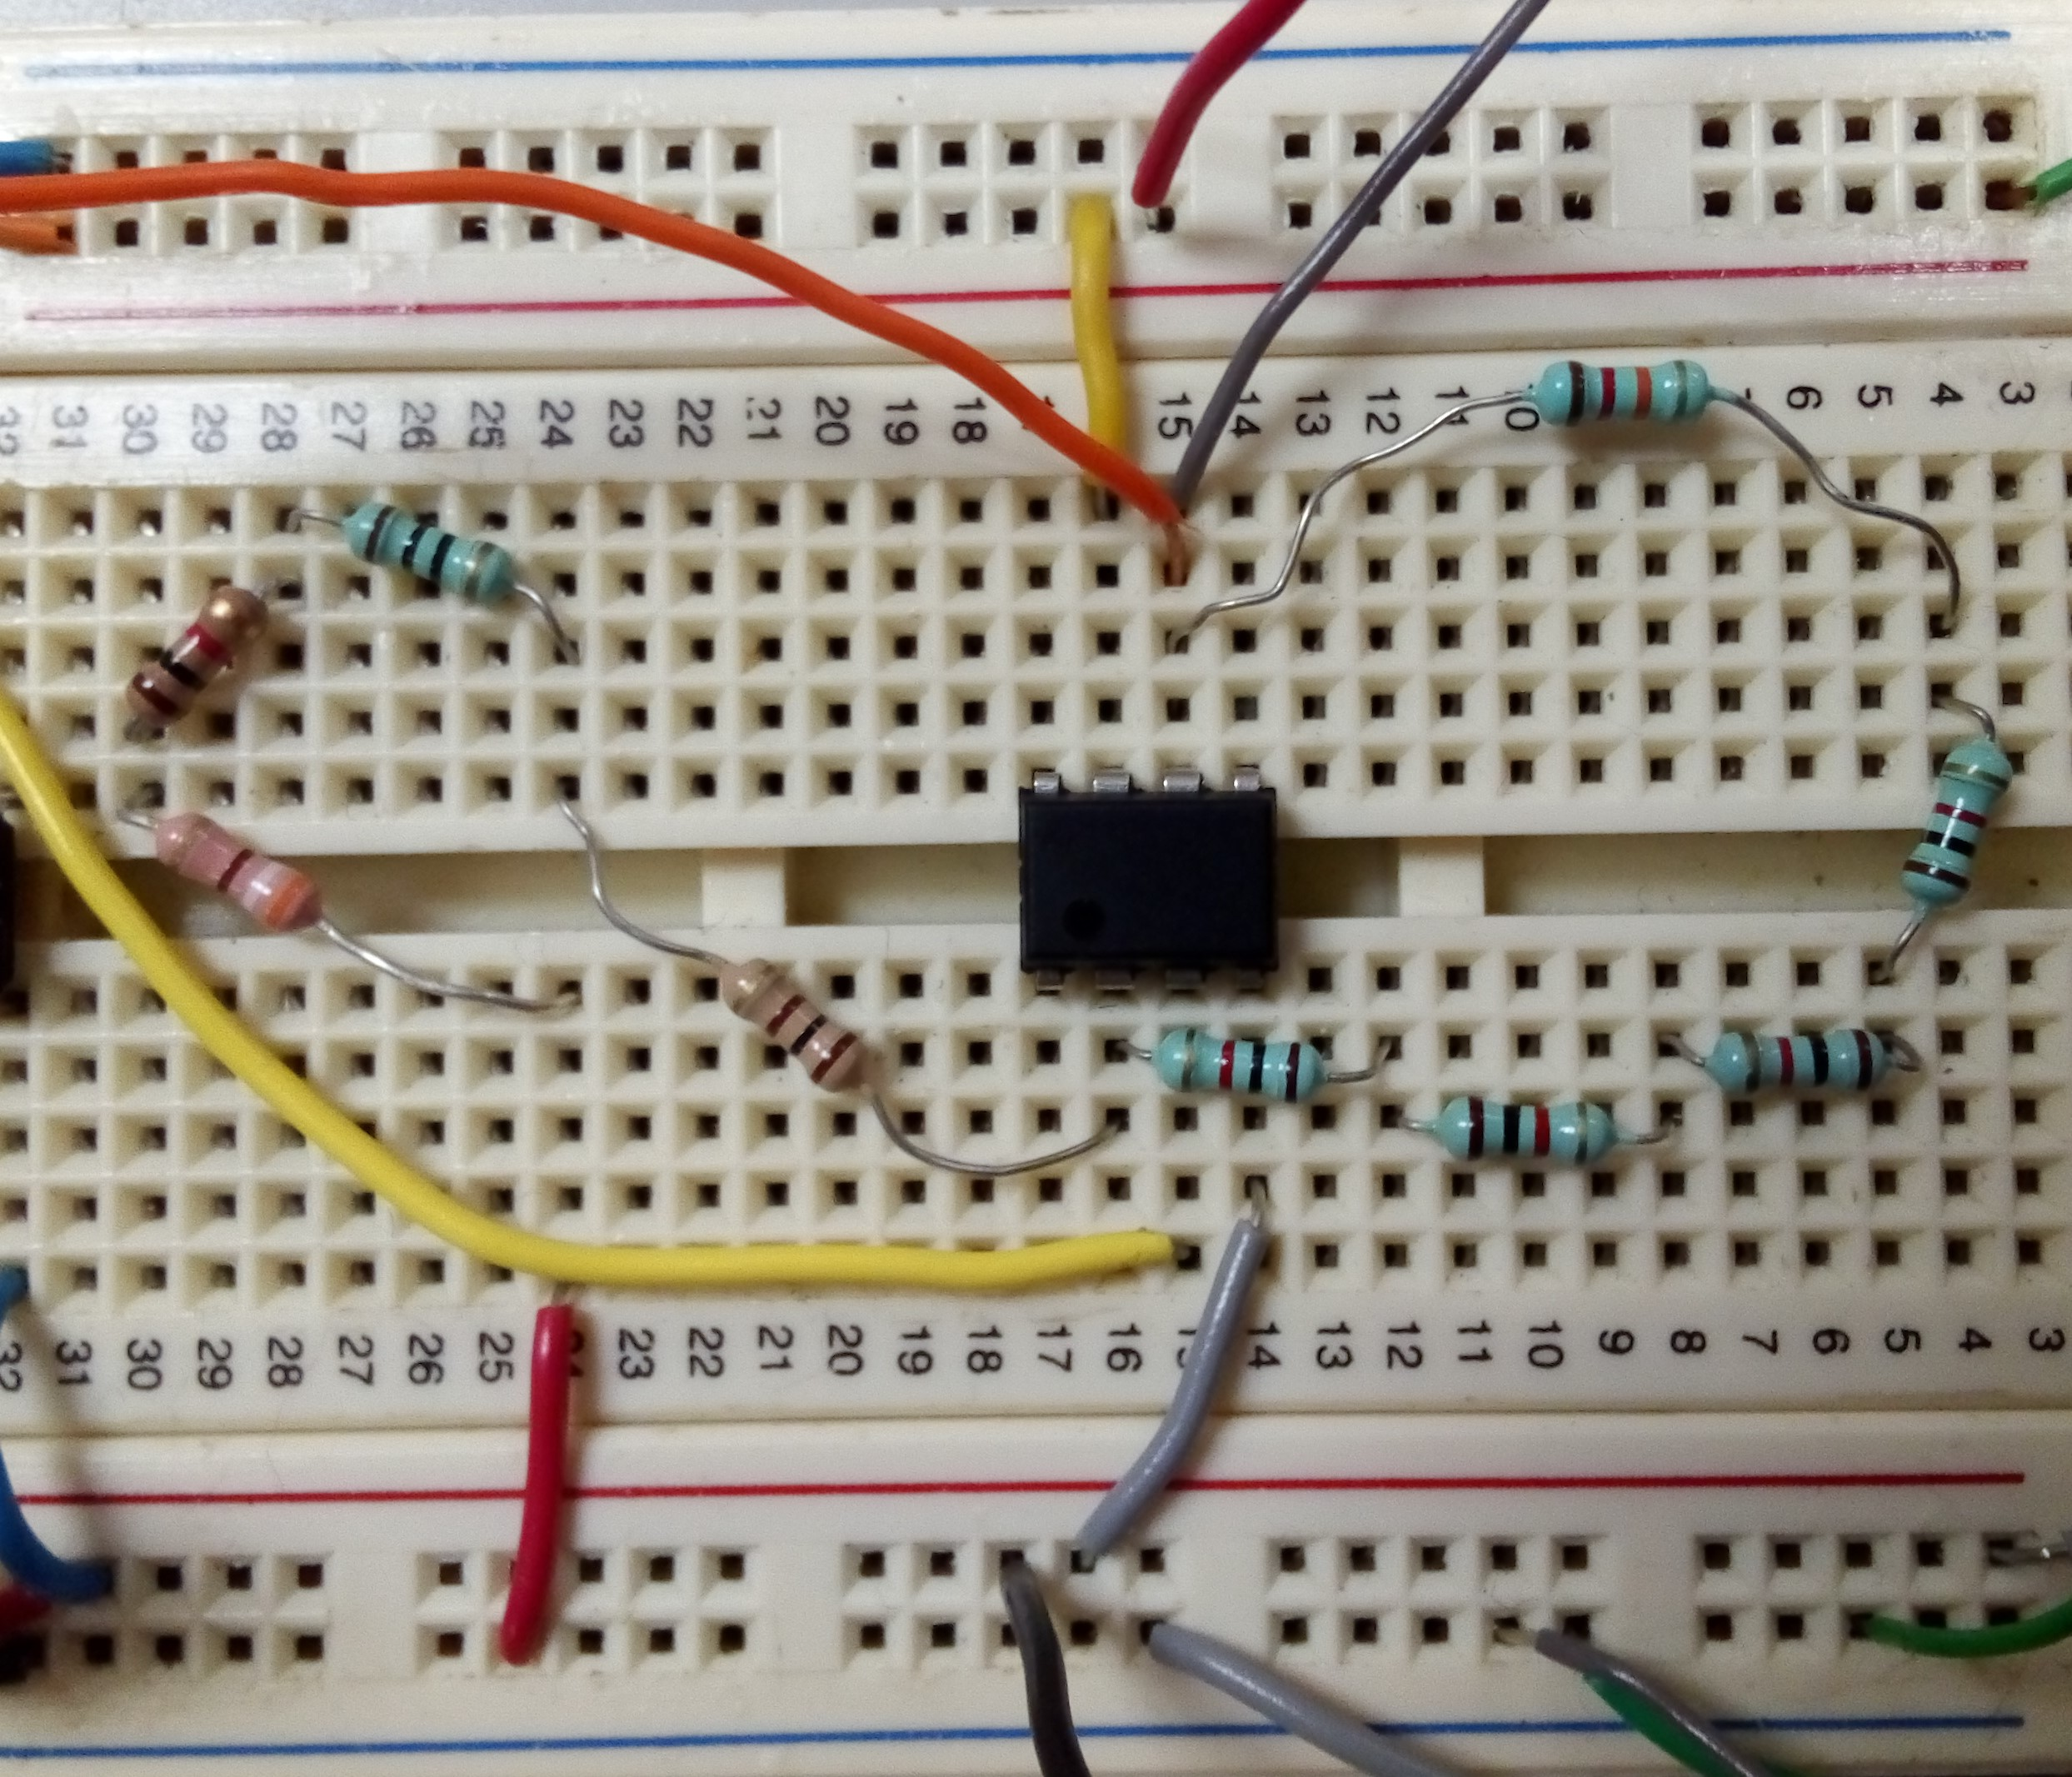
\includegraphics[width=0.7\textwidth]{Sismografo/Images/camplo2.jpg}
            \end{figure} 
            
	        \subsubsection{Medición de amplitud de señal - voltaje}
	        % -	Mida la oscilación máxima con el osciloscopio (Valor Vpp) e indíquela con unidades, respaldar la medición con la captura de pantalla e indique los parámetros de ajuste del osciloscopio (base de tiempo, volts por división, acoplamiento de señal), recuerde que la medición es simulando el movimiento con el cajón de prueba.
	        
	        \textbf{Parámetros de medición (Vpp)}
            \begin{multicols}{2}
                \begin{itemize}
                    \item[\checkmark] \textbf{Amplitud máxima de entrada: 880 mV}
                    \item[\checkmark] \textbf{Amplitud máxima de salida: 10.26 V}
                    \item[\checkmark] \textbf{Base de tiempo: 500ms}
            \columnbreak
                    \item[\checkmark] \textbf{Volts por división: 2 V}
                    \item[\checkmark] \textbf{Acoplamiento: Corriente Alterna}
                \end{itemize}
            \end{multicols}
            
            \textbf{Nota:} La linea amarilla es la señal del que sale del filtro y la azul la que sale amplificada a 10.26V.
	        % PONER FOTO DE LA MEDICIÓN HASTA LA ETAPA DE AMPLIFICACIÓN
	        \begin{figure}[h!]
                \centering
                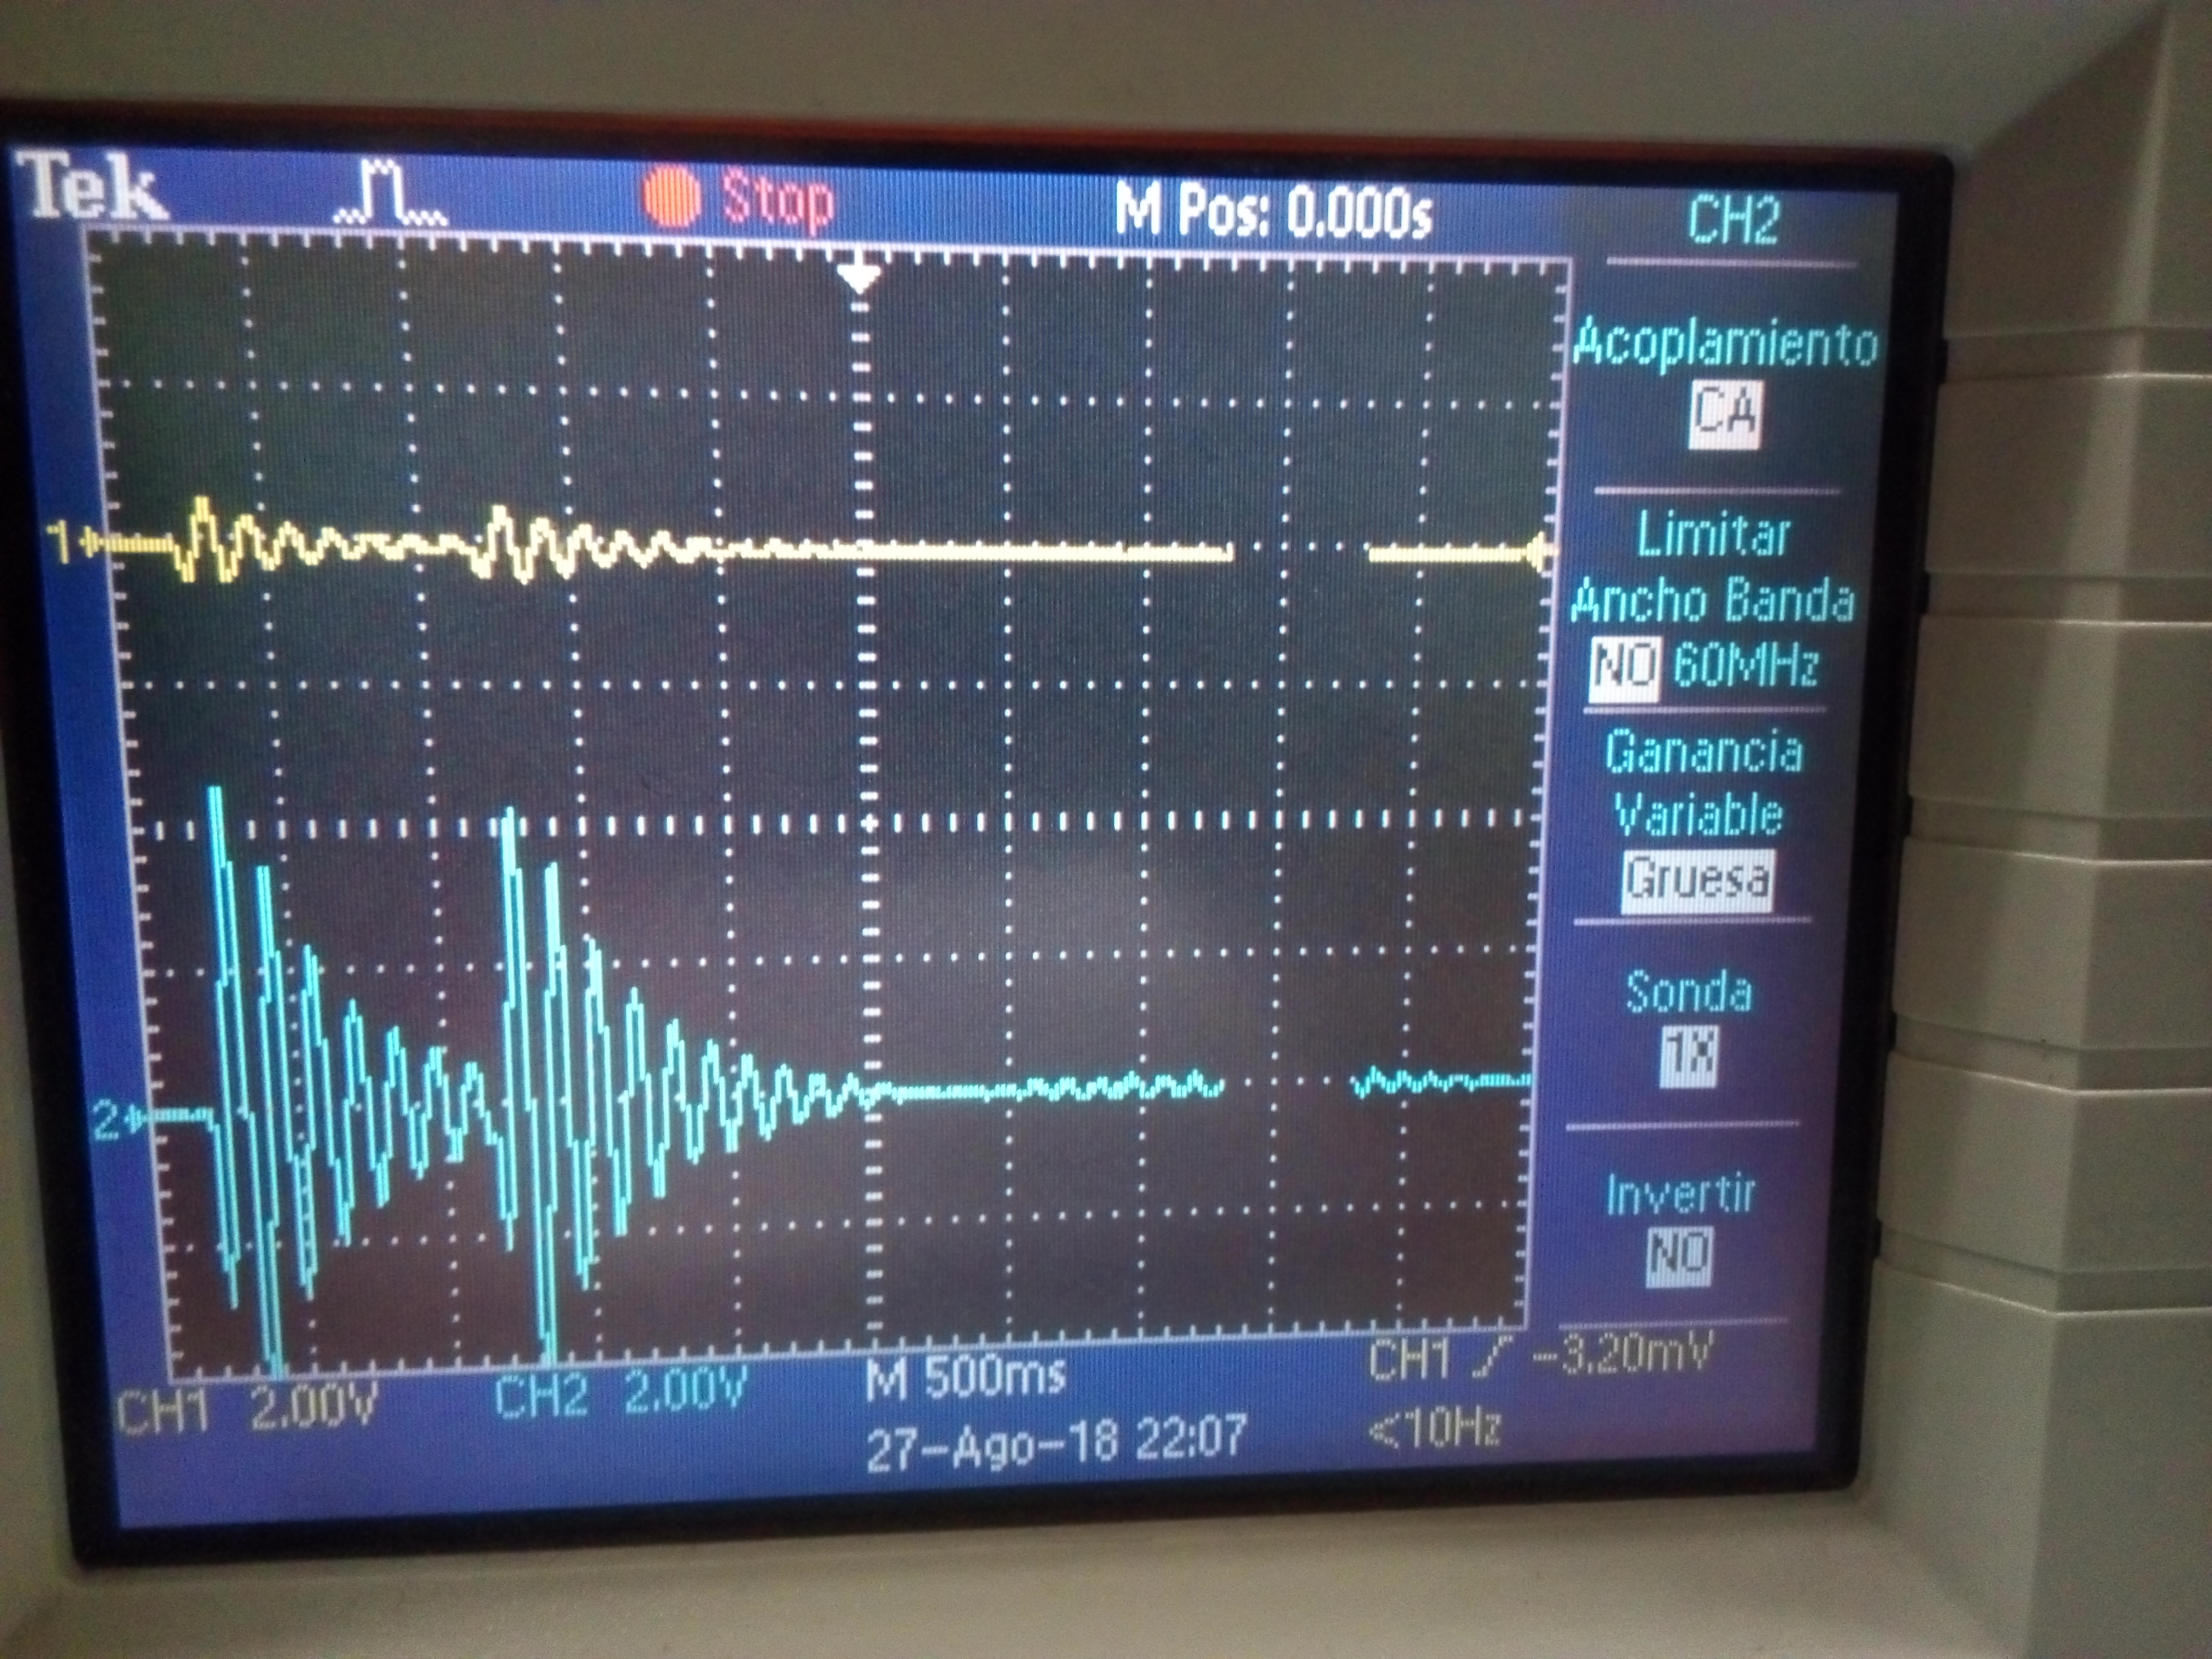
\includegraphics[width=0.7\textwidth]{Sismografo/Images/amplificada2.jpg}
            \end{figure} 
	       \newpage
	         \subsubsection{Explicación del funcionamiento de la etapa amplificadora}
	        % -	Explique cómo comprobó el funcionamiento de la etapa amplificadora.
	        El cambio es notable porque observamos en las mediciones que ambas están en la misma escala, y la señal azul sale amplificada, de esa forma nos dimos cuenta que nuestra etapa amplificadora estaba trabajando de manera correcta, con una ganancia de 11.66
	        \newpage
	    %/////////////////////////////////////////////////////////////////
    	%                   PROCEDIMIENTO EXPERIMENTAL 4
    	%/////////////////////////////////////////////////////////////////	        
	    \subsection{PE 4 - Empleo de un Vúmetro de led's como dispositivo indicador de intensidad}
	        
	        \subsubsection{Esquema}
	        % -	Haga un esquema de circuito completo del  Sistema que construyo, explique el funcionamiento iniciando desde el sensor (geófono) hasta el Vúmetro.
	        El siguiente circuito pertenece únicamente al vúmetro:
	        
	        % PONER ESQUEMA DEL CIRCUITO Vulmetro
	        \begin{figure}[h!]
                \centering
                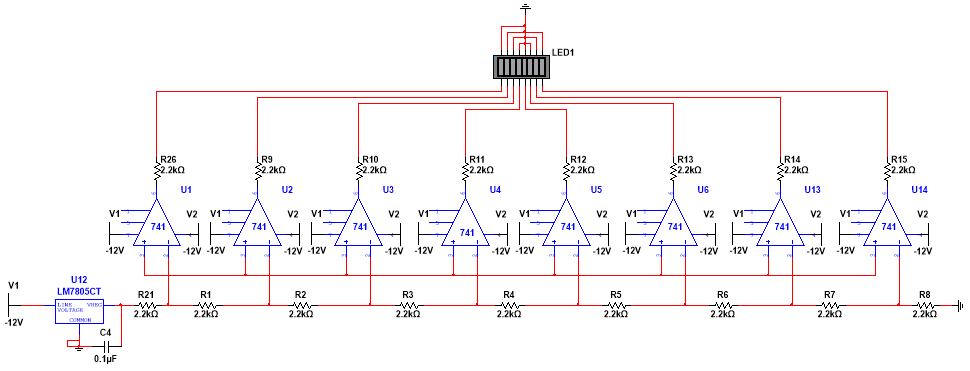
\includegraphics[width=\textwidth]{Sismografo/Images/vumetro.PNG}
            \end{figure} 
            
            \begin{figure}[h!]
            \subsubsection{Circuito cableado:}
                \centering
                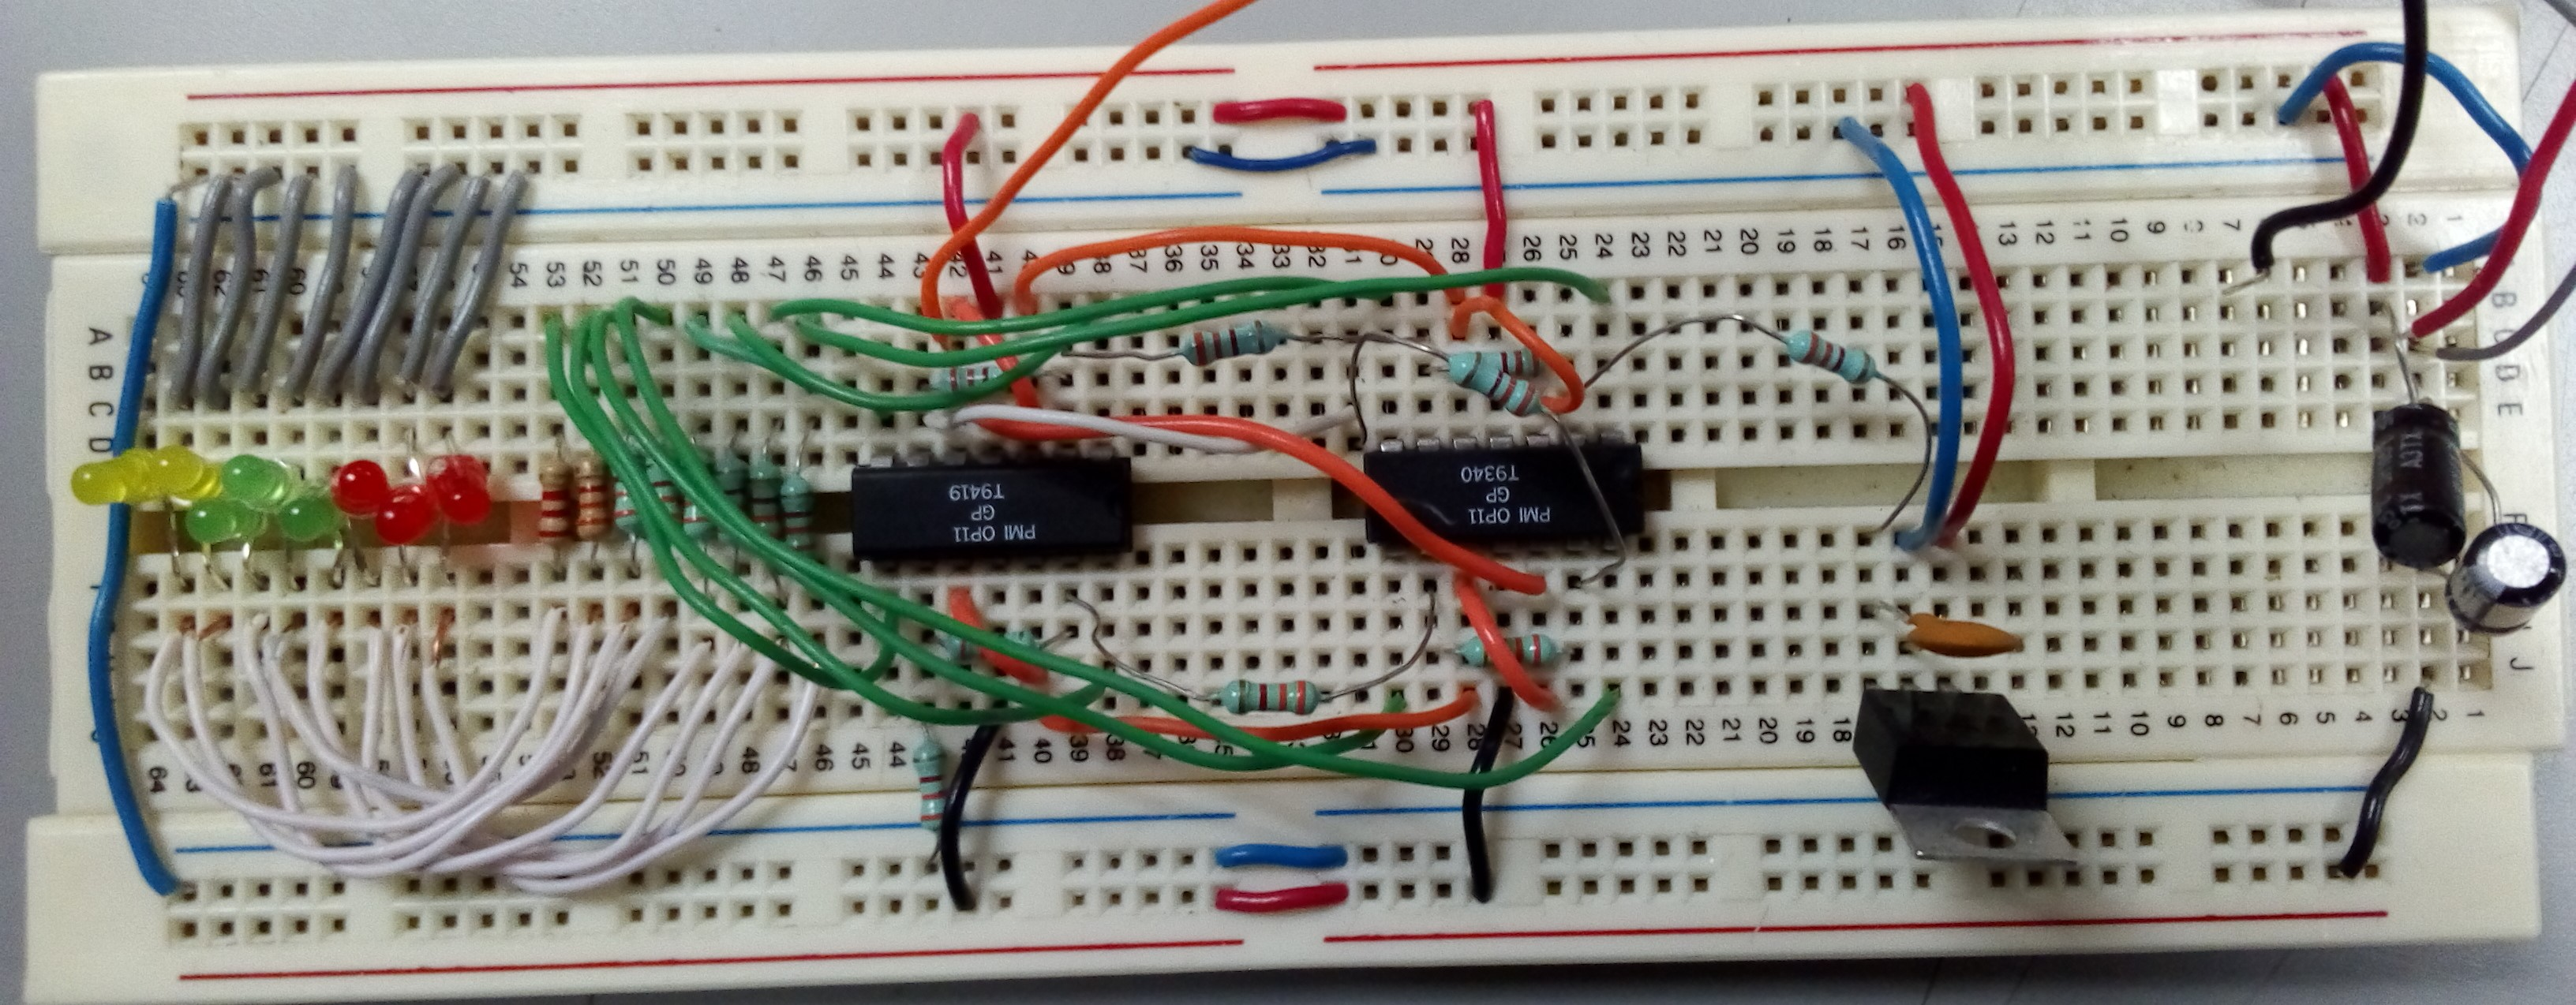
\includegraphics[width=\textwidth]{Sismografo/Images/cvumetro4.jpg}
            \end{figure}
            
            
            
            \newpage
            
            
            
	        \subsubsection{Funcionamiento del Vúmetro}
	        La señal de salida amplificada obtenida en la fase anterior se conecta en serie a las entradas no inversoras de los 8 amplificadores operacionales. Además, el voltaje de la fuente de alimentación pasa por un regulador de voltaje 7805 para estabilizarlo a 5V constantes, que irán directos a cada resistor de las entradas inversoras de los 8 amplificadores.
	        
	        De tal forma que se tiene un divisor de voltaje para reducir la amplitud de la señal de entrada. La señal varia de acuerdo a las variaciones del movimiento y hace que el arreglo de 8 LEDs enciendan de acuerdo al nivel de voltaje de la señal.
	        
	        En este caso, mientras más brusco sea el movimiento detectado por el sensor, la bocina rebotará con más fuerza, enviando una señal con la amplitud máxima que viajara hasta el vúmetro, provocando que los LEDs que enciendan emulando una escala del verde (movimiento leve) al rojo (movimiento fuerte).
	        
	        Los siguientes datos se justifican en la sección de anexo: 
	        
	        \textbf{Rango de medición (voltaje):} $0.55 V$ a $4.44 V$
	        
	        \textbf{Resolución (voltaje):} $0.55 V$
	        
	        \subsection{Circuito completo en ejecución}
	        El esquema del circuito completo es el siguiente:
            % PONER ESQUEMA DEL CIRCUITO COMPLETO
	        \begin{figure}[h!]
                \centering
                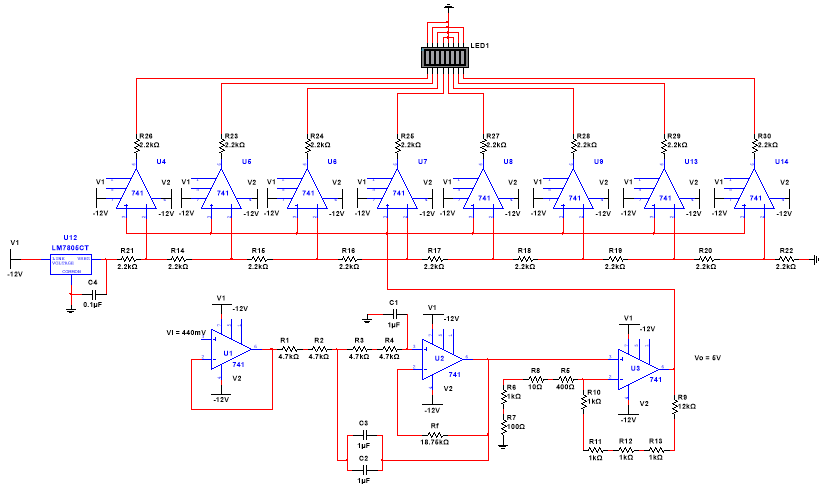
\includegraphics[width=1.05\textwidth]{Sismografo/Images/circuito.PNG}
            \end{figure} 
            \newpage
            \textbf{Circuito completo cableado:}
            \begin{figure}[h!]
                \centering
                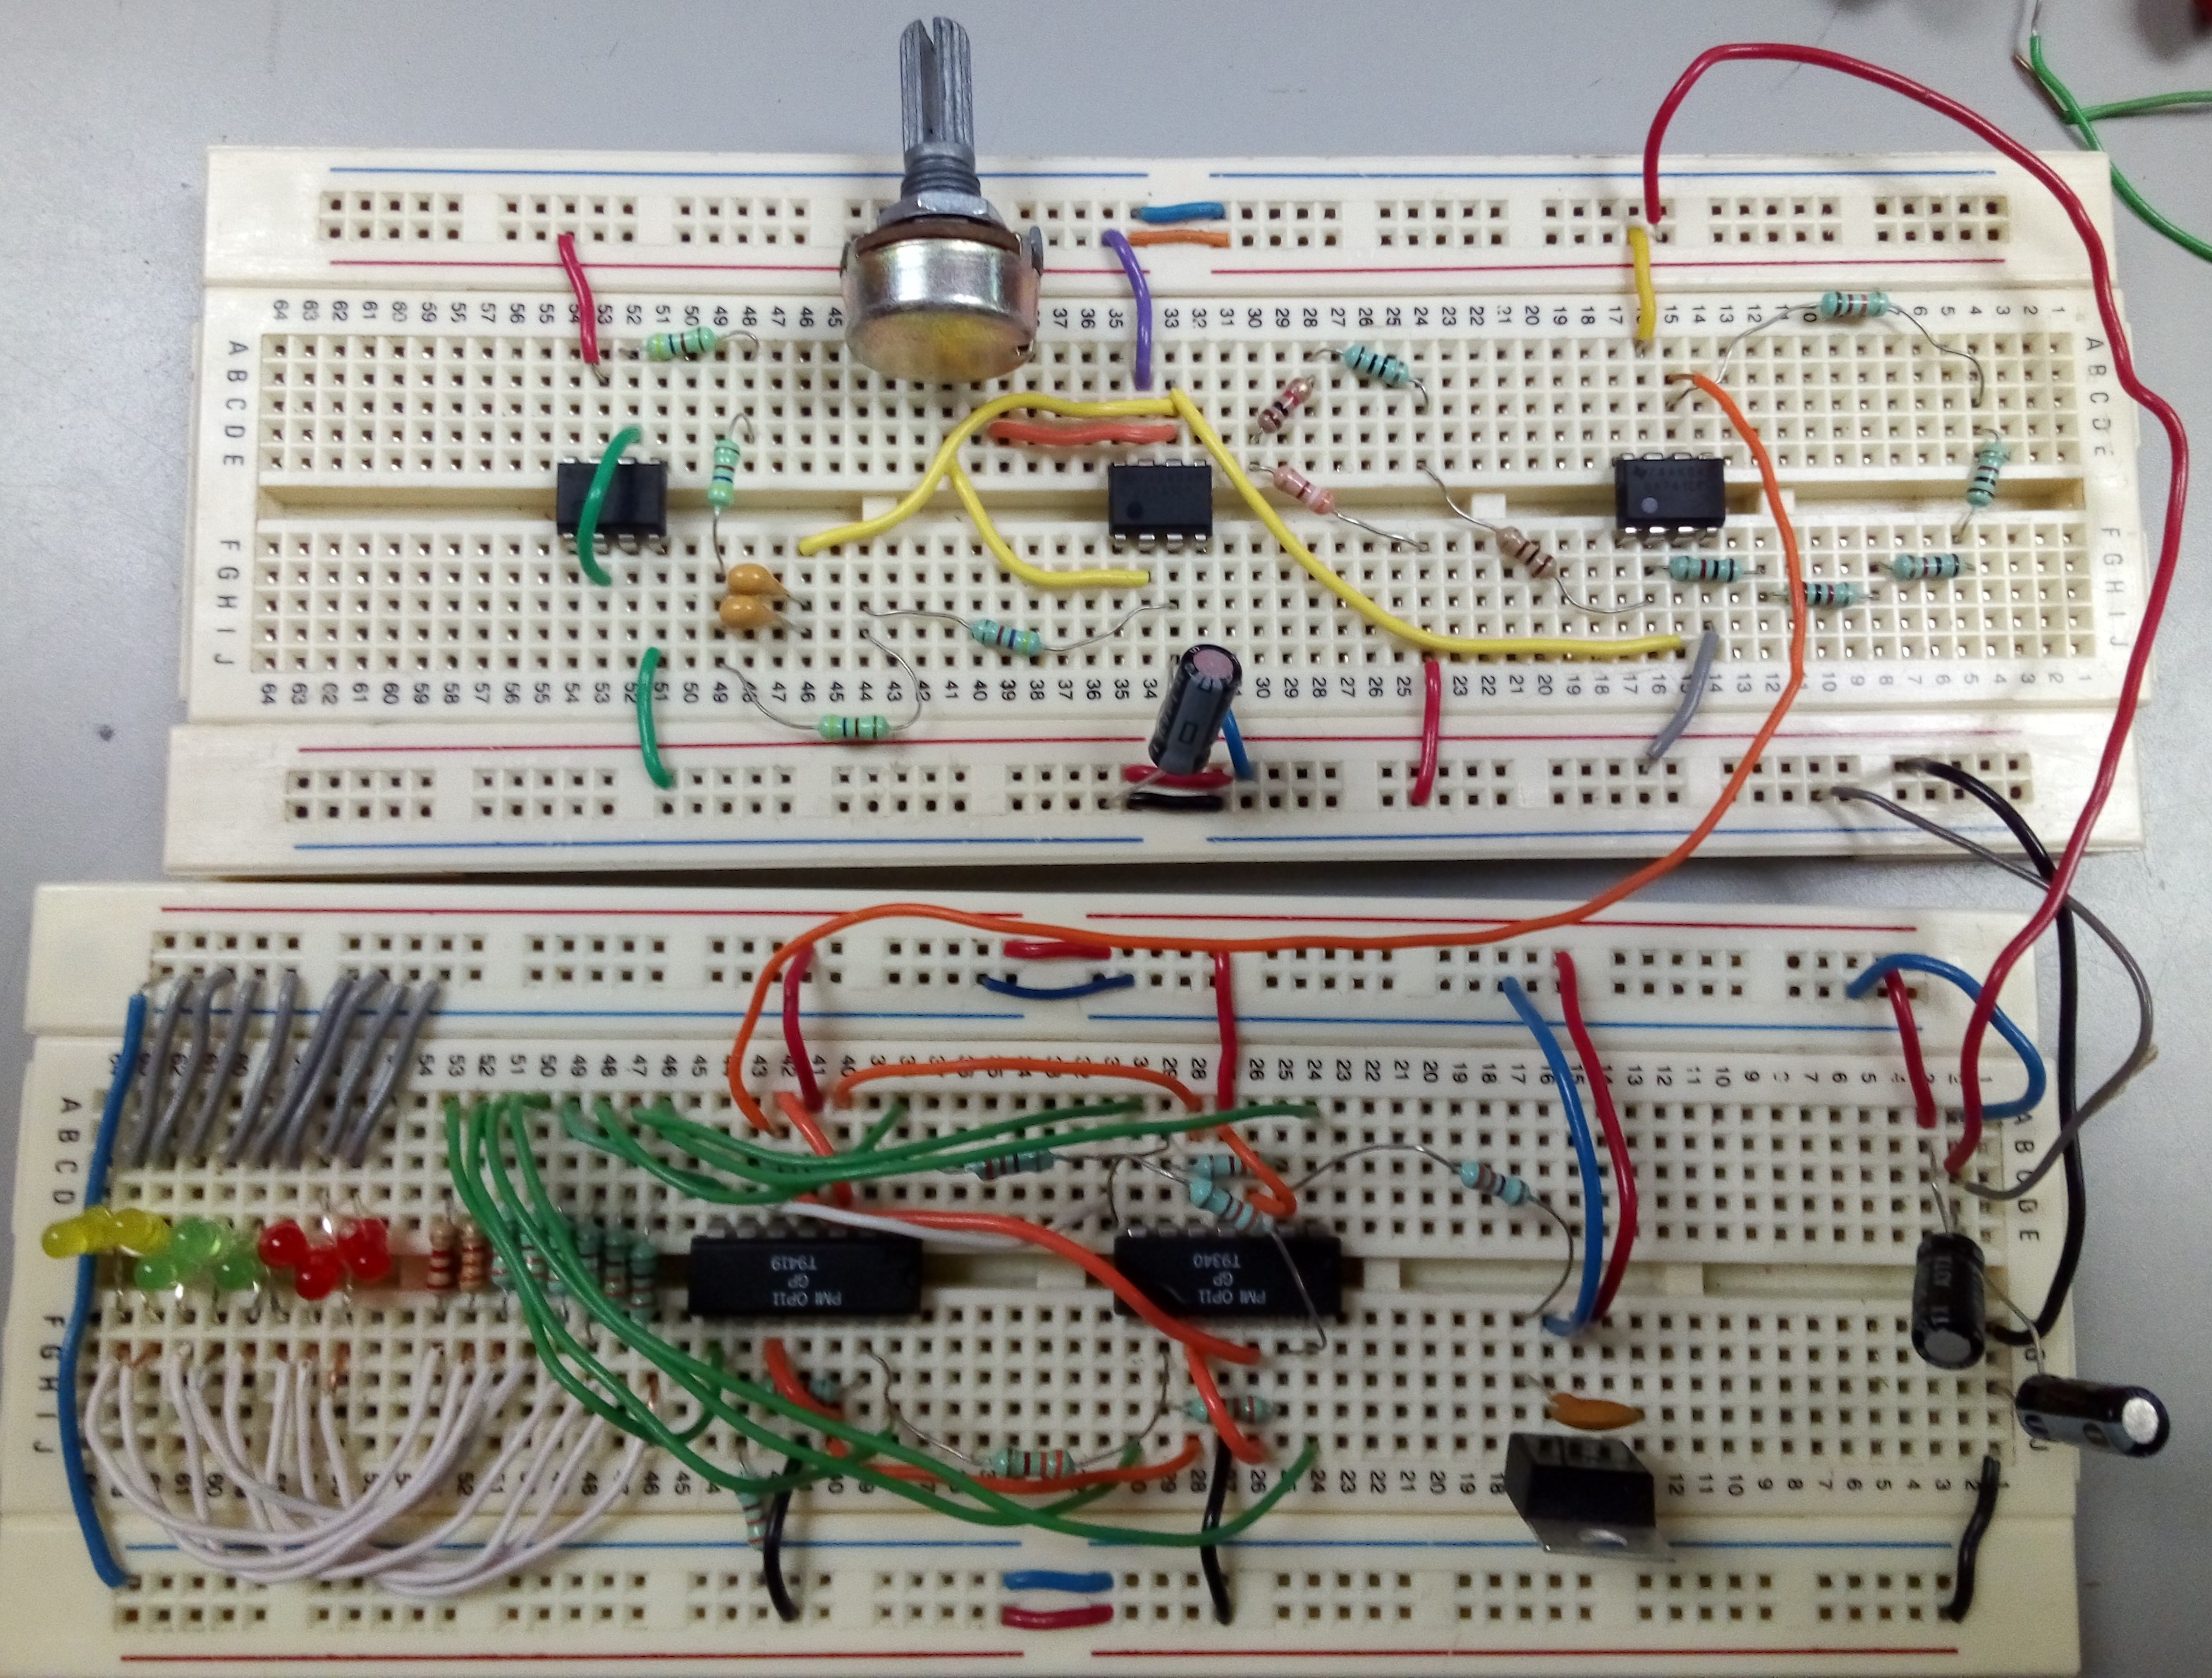
\includegraphics[width=0.75\textwidth]{Sismografo/Images/proto1.jpg}
            \end{figure} 
            
           \textbf{ Al aplicar un movimiento en el geófono encienden los LEDs:}
            \begin{figure}[h!]
                \centering
                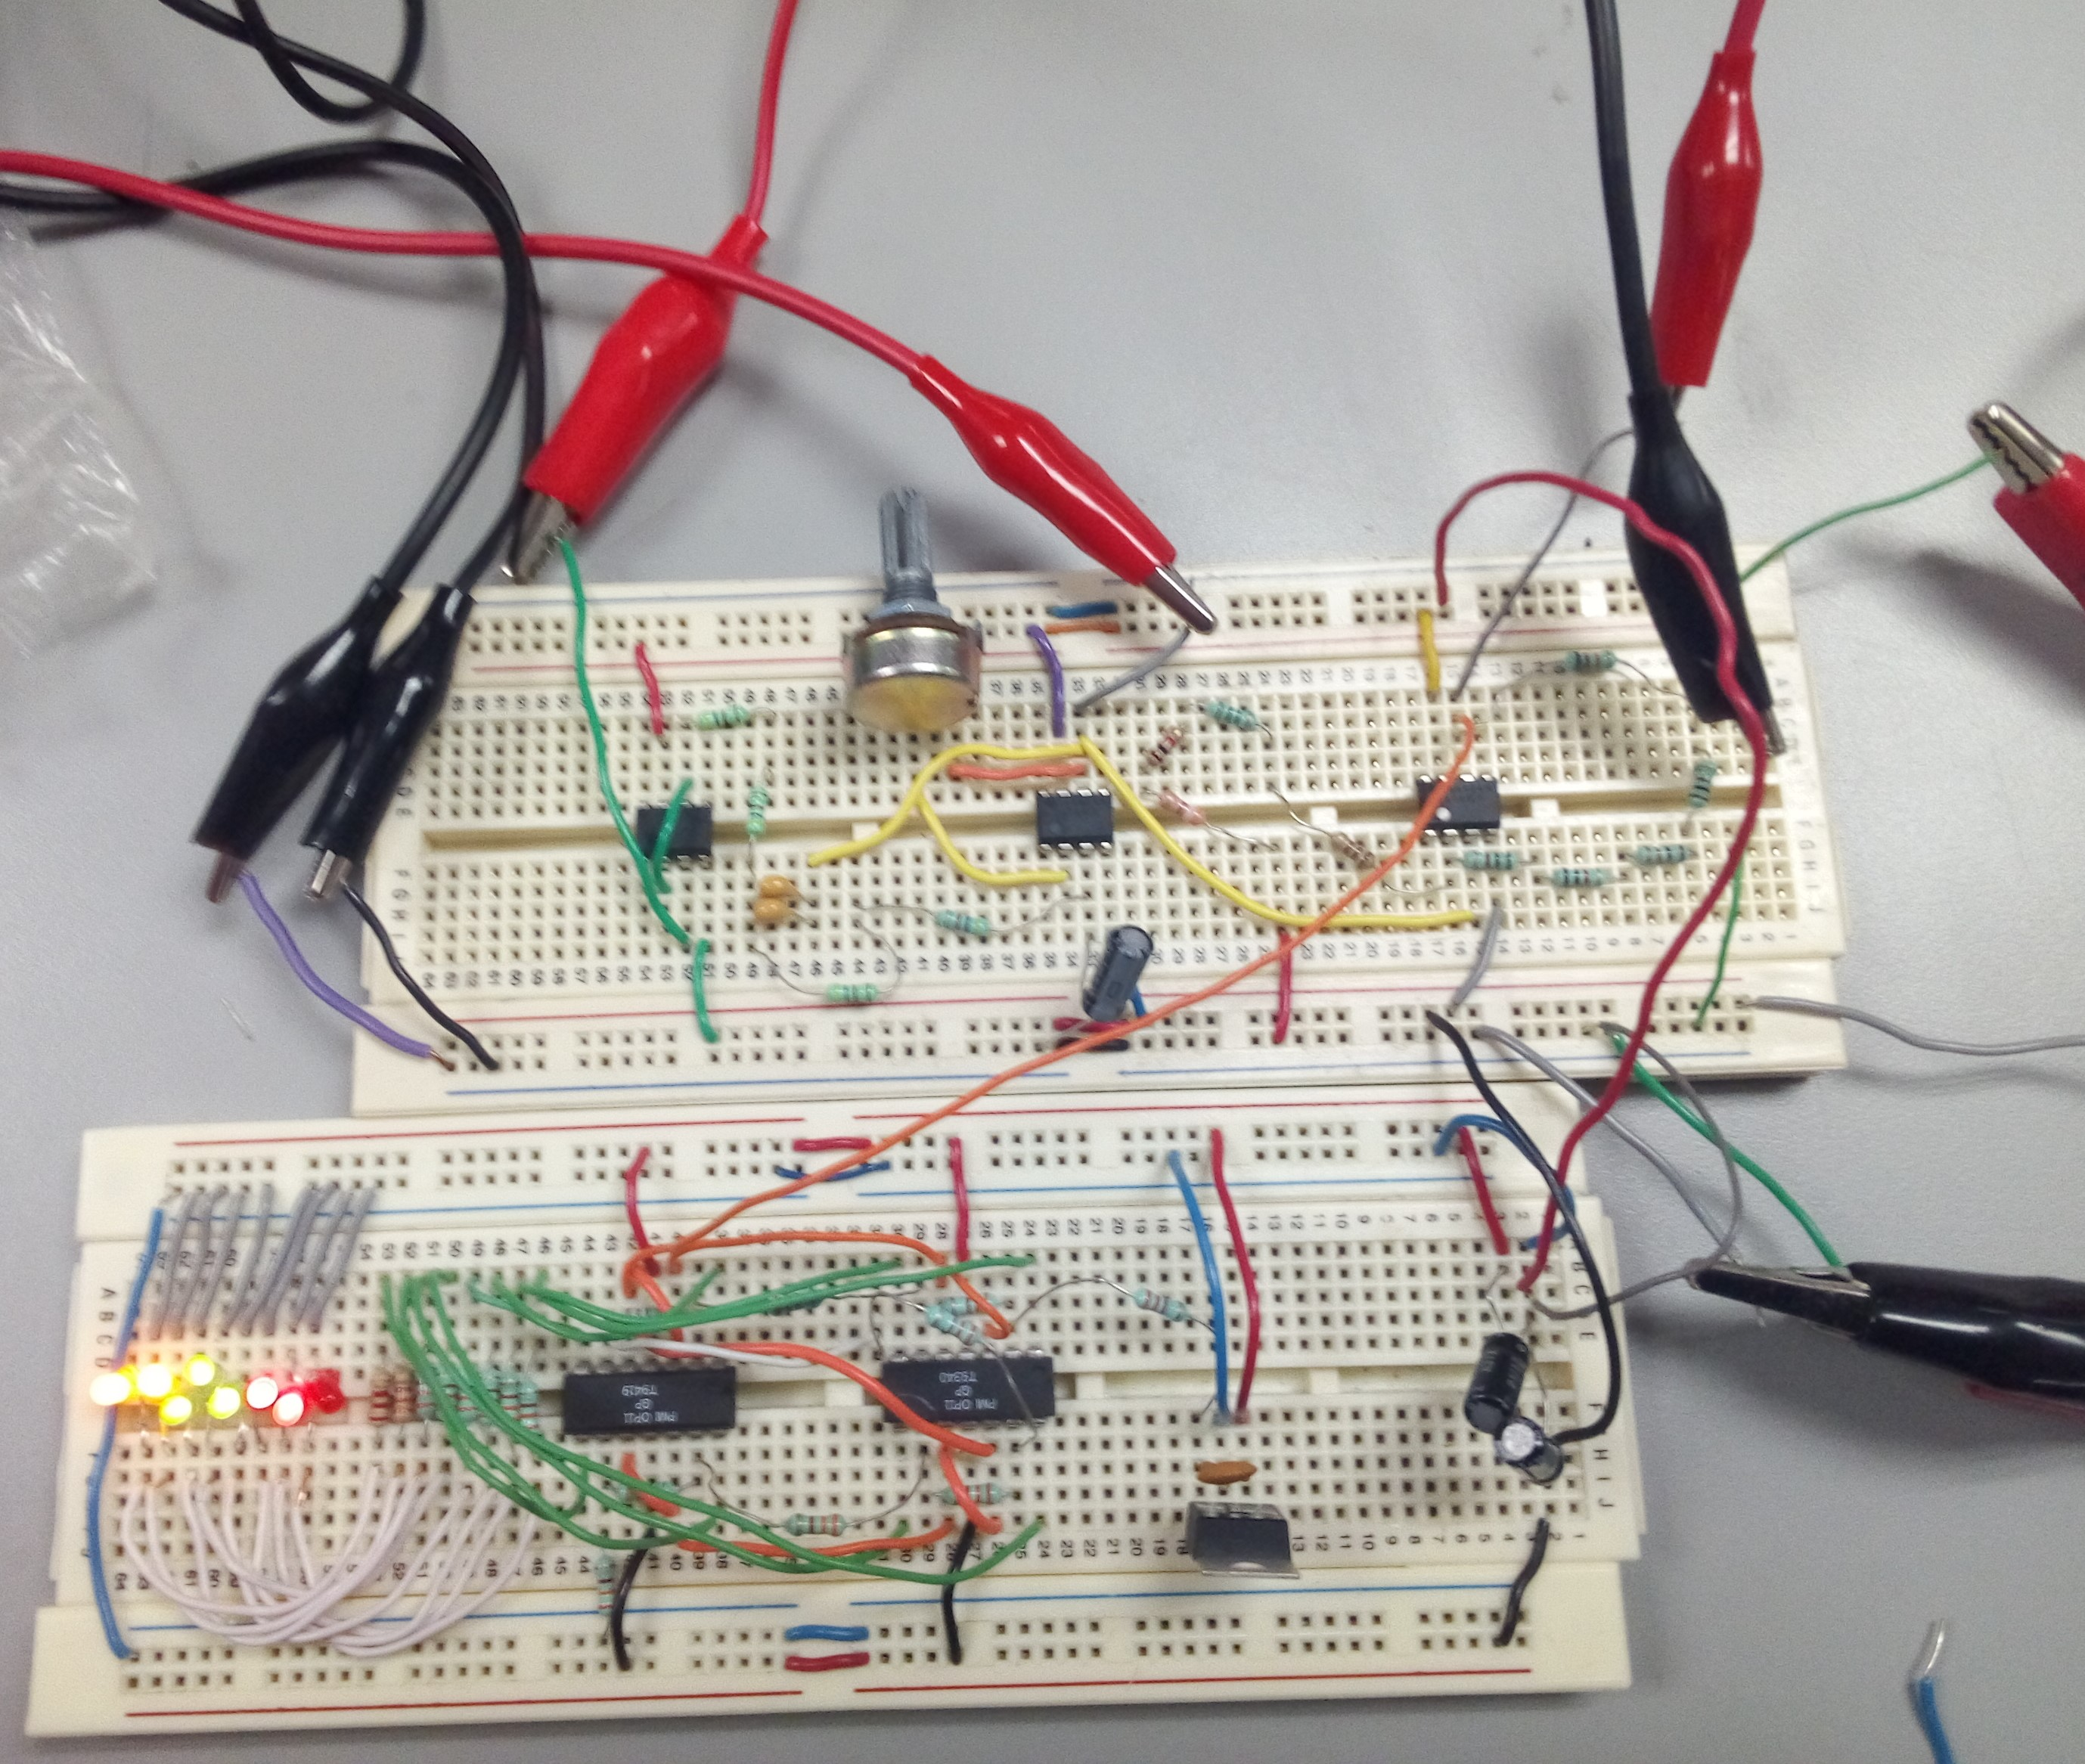
\includegraphics[width=0.75\textwidth]{Sismografo/Images/proto8.jpg}
            \end{figure} 
            
            \textbf{Vista completa:}
            \begin{figure}[h!]
                \centering
                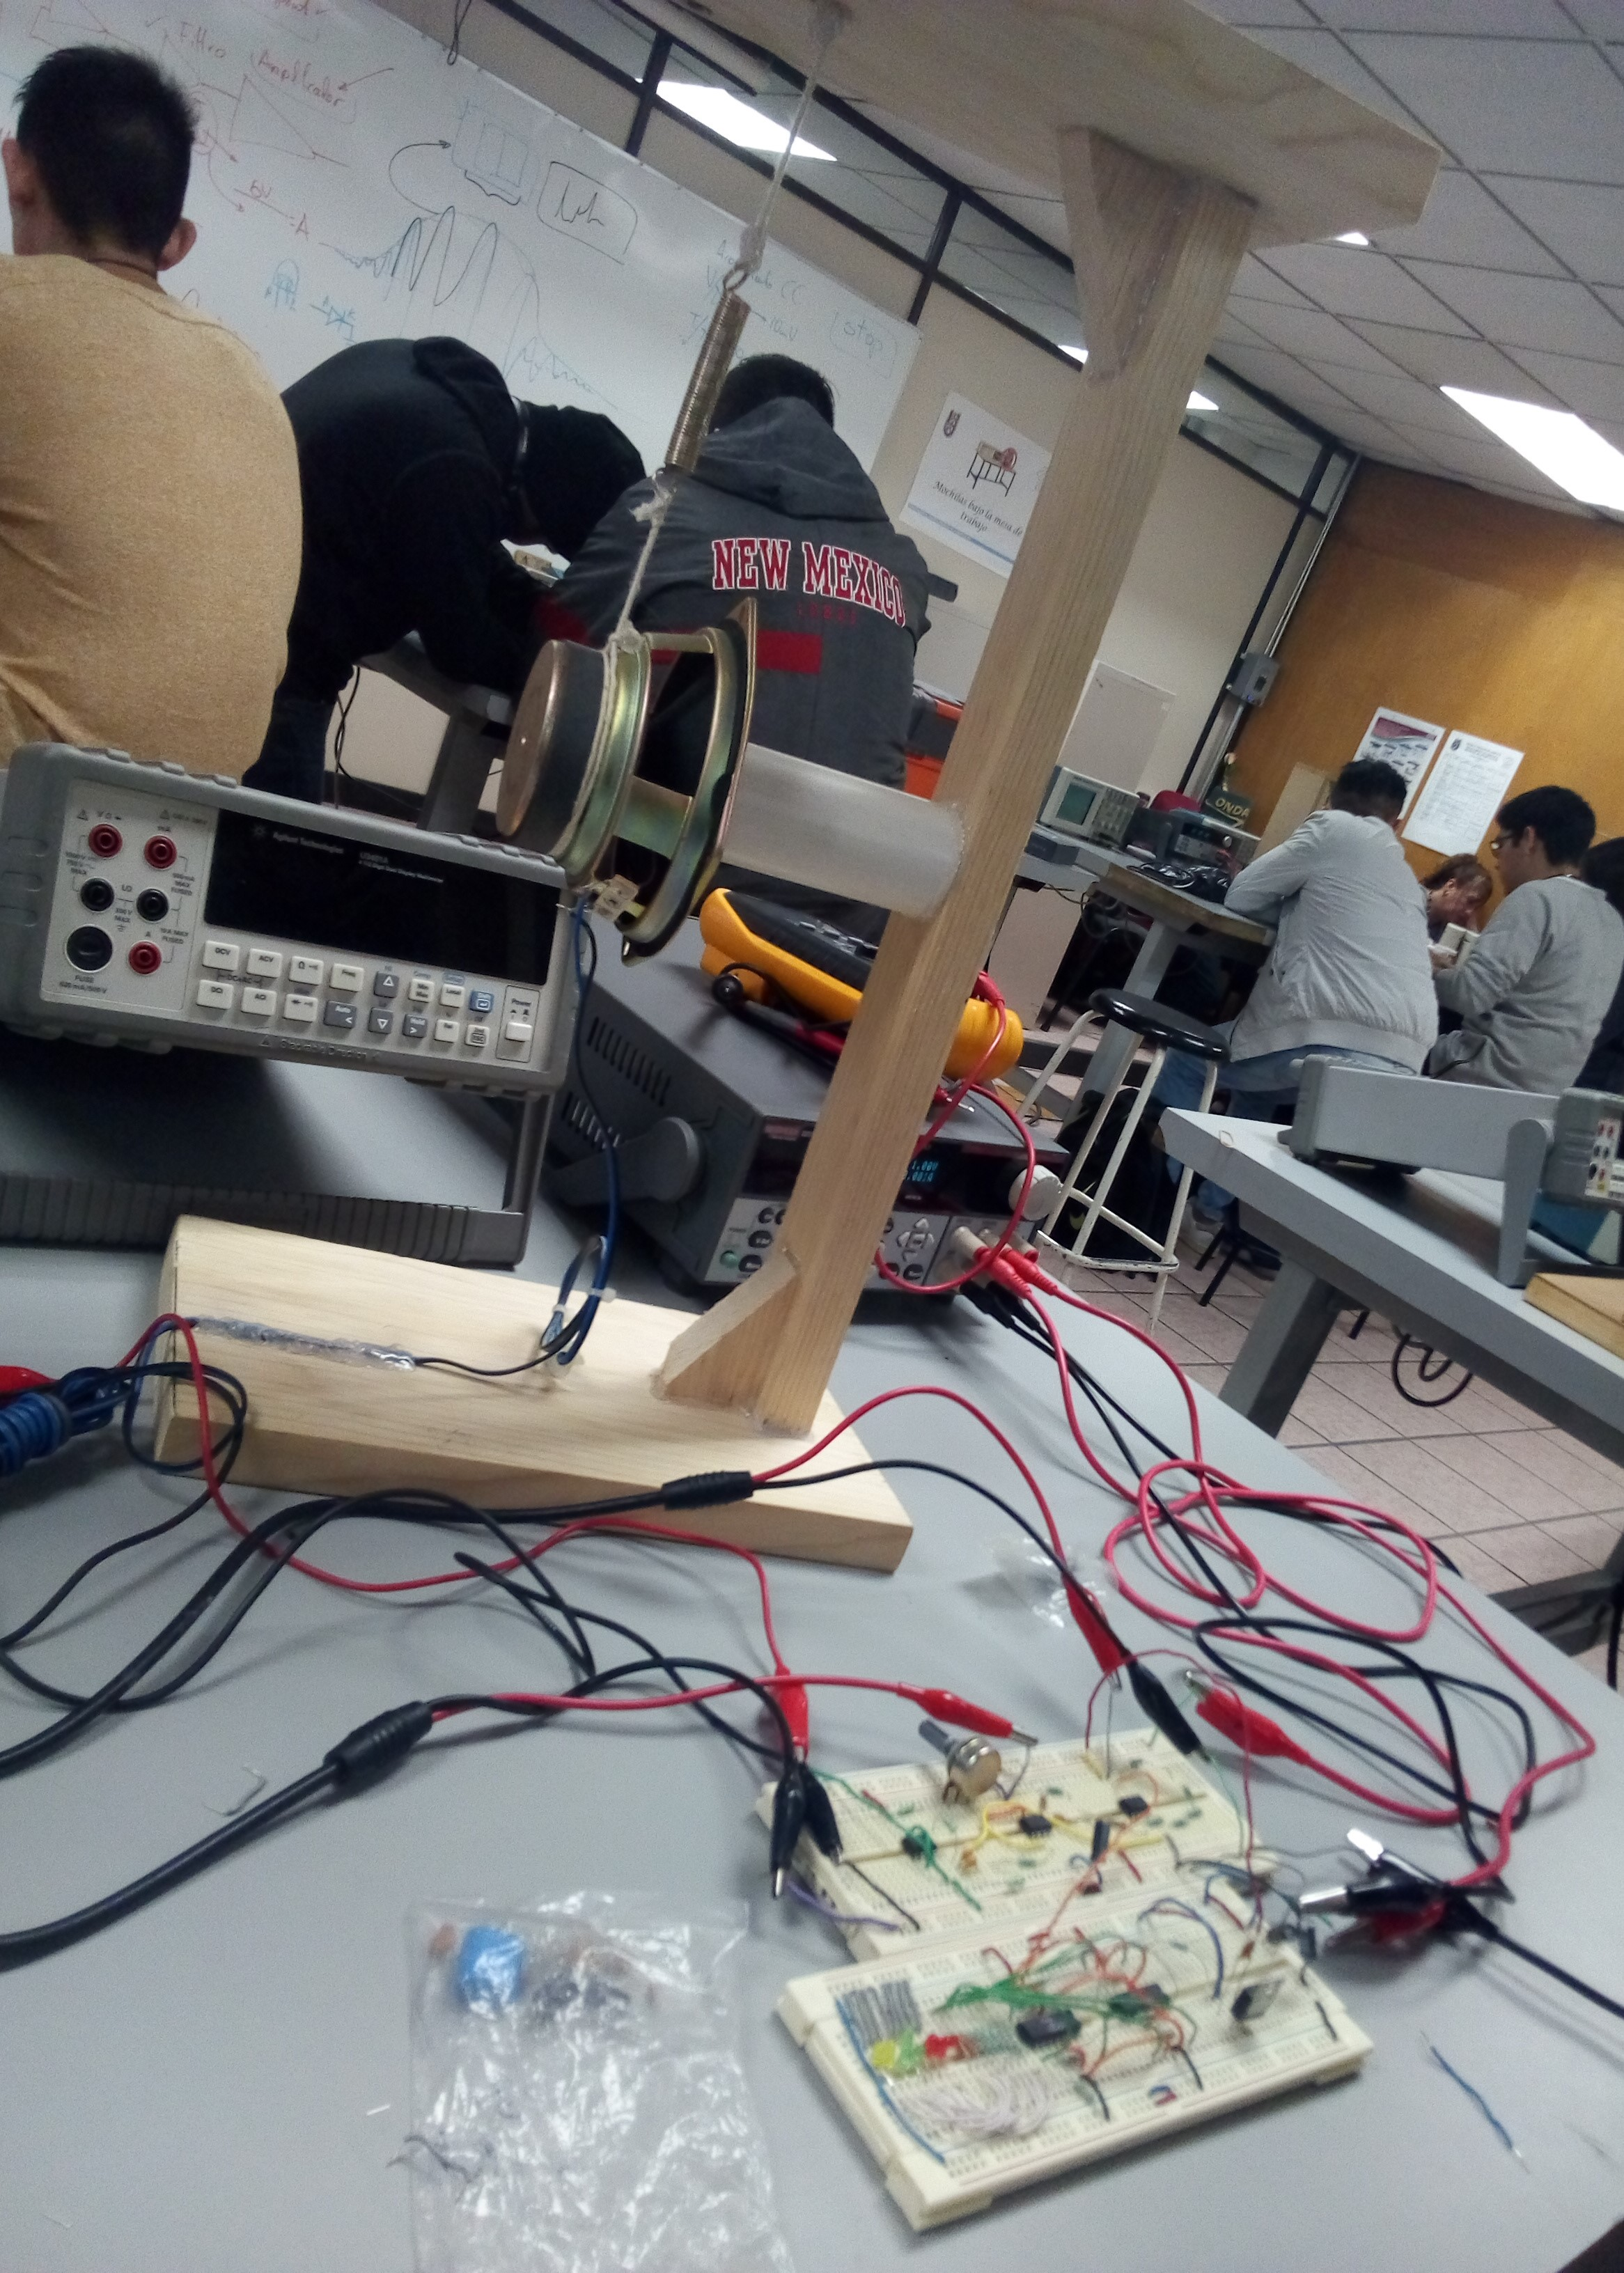
\includegraphics[width=0.6\textwidth]{Sismografo/Images/c1.jpg}
            \end{figure} 
            \subsubsection{Explicación del funcionamiento del circuito completo}
	        % -	Explique cómo comprobó el funcionamiento de la etapa amplificadora.
	        Al aplicar un movimiento al sensor geófono, la señal con amplitud máxima de 880 mVpp viaja por los cables conectados en la bocina hasta el primer amplificador, el buffer, que adapta el nivel de salida de alta impedancia del géofono, al filtro con un nivel de entrada de baja impedancia.
	        
	        Entramos a la segunda fase, la del filtrado, en donde nuestra señal ya esta acoplada pero aun posee picos de ruido muy altos. Al entrar al filtro este limita la frecuencia de la señal a una frecuencia menor a 12 Hz.
	        
	        Ya limpia nuestra señal y a prueba de detección de señales de un origen ajeno a un sismo, es momento de amplificarla a 10Vpp, al orden de los volts en donde es más sencillo y práctico medir. Esto ocurre al entrar a la tercera fase del circuito: la segunda etapa de amplificación. La señal de entrada de 880 mVpp se convierte en una de aproximadamente 10.26 Vpp.
	        
	        Finalmente, ya con nuestra señal acoplada, filtrada y amplificada la enviamos a un arreglo de 8 amplificadores operacionales con un LED en cada uno, llamado vúmetro. 
	        
	        La señal de salida amplificada obtenida en la fase anterior se conecta en serie a las entradas no inversoras de los 8 amplificadores operacionales. 
	        
	        Además, el voltaje de la fuente de alimentación pasa por un regulador de voltaje 7805 para estabilizarlo a 5V constantes, que irán directos a cada resistor de la entradas inversoras de los 8 amplificadores.
	        
	        Por medio de un divisor de voltaje, esta fase servirá para establecer una resolución, que fue de 0.55V, y el rango de medición resulto de 0.55 V a 4.44 V
	        
	        Según la amplitud de la señal recibida, se irán encendiendo del LED más a la izquierda hacia el LED más a la derecha, reflejando la intensidad del movimiento captado por el sensor, similar a cuando se mide el volumen de algún sonido en un ecualizador. La sección de amarillo (0.55V) significa movimiento leve y la de rojo (4.44V) significa movimiento altamente brusco.
	        
	      
    
            \newpage
	        \subsubsection{Diagrama bloques}
	        % -	Dibuje un diagrama a bloques  que represente a su sistema de medición e indique cuales elementos de circuito corresponden a cada etapa.
	        
	        \begin{figure}[h!]
                \centering
                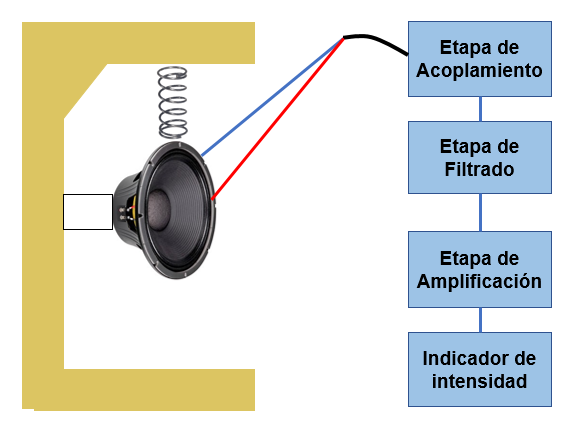
\includegraphics[width=0.7\textwidth]{Sismografo/Images/DiagramaBloques.PNG}
            \end{figure}
	        \subsubsection{Posibles mejoras}
	        El geofóno realizado tiene un buen funcionamiento, sin embargo, como es sabido, todo se puede perfeccionar, algunas de las mejoras que se pueden realizar a este instrumento son:
	        \begin{itemize}
	            \item Colocar tubos, bocinas y resortes en otras partes del instrumento, en distintas posiciones no solo en una dirección, de tal forma que sea más sensible a los movimientos sísmicos, tanto sismos de movimiento oscilatorio (diseño actual), como sismos de movimiento trepidatorio (bocina extra en posición vertical). 
	            \item Enviar la señal generada a una aplicación por medio de un módulo de Arduino, en la cual se podrá ver la intensidad del sismo en escala Richter y notifique a algún dispositivo del usuario (celular, laptop, computadora, pantalla LCD, etc.) por medio de un módulo Bluetooth de dicha aplicación acerca del movimiento sísmico que está ocurriendo, además de mostrar la señal del comportamiento del movimiento.
	            
	            \item La aplicación puede ser desarrollada con arduino, con "The Arduino IDE", el cual no solo está desarrollado en Java, sino que, como es lógico de pensar, puede comunicarse con ayuda de este lenguaje de programación, con la librería RXTX Java Library. 
	            
	            \item Diseñar y añadir un filtro pasa altas al filtro de la segunda etapa experimental, para acotar de una forma más precisa la frecuencia que deseemos medir, completando así el \textbf{filtro de banda}.
	            
	        \end{itemize}
	        
	        % -	Explique cómo podría mejorar el funcionamiento de su Sistema de Medición.
	        
\newpage

	%/////////////////////////////////////////////////////////////////
	%							CONCLUSIONES INDIVIDUALES
	%/////////////////////////////////////////////////////////////////
	\section{Conclusiones}
	    \subsection{Arianna Itzamina Aguilar Herrera}
	    La realización de esta práctica tenía varios fines, entre ellos dar un repaso de lo que fue la materia de ''Electrónica Analógica'', objetivo que fue cumplido, pues no solo se repasaron conocimientos, sino que se reafirmaron e incluso se aprendieron.
	    
	    Por ejemplo se reafirmo en uso de los amplificadores operacionales, tanto como buffer como amplificador no inversor.
	    
	    En mi caso el tema de filtros en su momento lo comprendí, aunque no me quedaba del todo claro, después de haber realizado esta práctica puedo decir que ya lo sé. 
	    
	    Además, se aprendieron cosas nuevas, como teoría sísmica, que si bien podría decirse no es propiamente parte de la materia, pensándolo a fondo lo es, pues maneja conceptos propios de la materia, además, es algo que podemos medir, para lo cual necesitamos un instrumento de medición, y eso es lo que aprendemos en instrumentación, encontrar una variable que se pueda medir, y crear instrumentos para medirlos, así pues, el geófono es un buen instrumento, para repasar, reafirmar y aprender sobre la materia. 
	    \subsection{Nicolás Sayago Abigail}
	    Al finalizar esta práctica pude tener retroalimentación en bastantes temas que mencionare a continuación:
	    \begin{itemize}
	        \item[\checkmark] La teoría sísmica jamás la había leído, sin embargo es interesante notar las frecuencias que suelen tener los sismos y como la teoría te ayuda a hacer planteamientos para generar un circuito, en este caso que nuestro filtro fue con 12 Hz de frecuencia.
	        
	        \item[\checkmark] La aplicación que le dimos a los filtros me ayudo a entender bastante su función, cuando filtramos una señal podemos hacer que nuestro objetivo de analizar cierta señal sea parcialmente limpia, en este caso es importante puesto que para que nuestro sismógrafo sea lo más exacto posible debe \textbf{filtrar} cosas innecesarias.
	        
	        \item[\checkmark] Al amplificar la señal note que es importante para poder observarla de manera correcta y hacer que los voltajes pequeños sean mayores de tal forma que podamos usarlos después, en este caso para el vúmetro.
	        
	        \item[\checkmark] Finalmente el vúmetro y sus cálculos me ayudaron a recordar principios básicos de análisis de circuitos. Además que esta ultima etapa es la parte que ayuda a interpretar la intensidad de los sismos, lo cual es bastante útil para darle más usos si así se desea.
	    \end{itemize}
	    
	    \subsection{Ramos Diaz Enrique}
	    La idea de realizar un sensor sísmico por medio de circuitos eléctricos a partir de elementos tan sencillos como resistencias, capacitores y amplificadores operacionales me parecía imposible antes de ésta práctica.
	    
	    Al investigar sobre la teoría sísmica me tope con muchos conceptos y fenómenos que se manejan dentro de la electrónica: frecuencia, onda, intensidad, campo electromagnético, ruido, además de unos cuantos revisados en la propia clase de la materia: rango, medición, escala.
	    
	    Una vez construido y entendido el funcionamiento del geófono casero, comprendí la importancia de cada una de las etapas y comprendí el objetivo de sus componentes.
	    
	    Por ejemplo, con el buffer el fin era de cierto modo proteger nuestra señal y circuito completo, aislándolo y amortiguándolo para que la potencia de entrada se altere muy poco. 
	    
	    El diseño del filtro fue algo complicado, pues decidimos cablear uno de segundo orden que incluye más resistencias que las del diseño propuesto y un primer amplificador operacional extra. A pesar de esto, el resultado fue el esperado, pues eliminamos todo el ruido no deseado que el sensor detecta en el medio, como golpes en la superficie o pasos al caminar.
	    
	    Al amplificar la señal no hubo complicaciones, pues exitosamente logramos alcanzar los 10V en la salida.
	    
	    Pero incluso después de todo esto esa señal no tenia un significado, por lo que la idea del vúmetro se me hizo muy divertida. Emulamos un semáforo con los colores verde, amarillo y rojo e inventamos una pequeña escala a la cual le dimos un significado un poco abstracto.
	    
	    Este tipo de prácticas son muy útiles para llamar la atención de aquellos a los que no les agrada la electrónica en general, pues de forma implícita maneja conceptos como diseño de filtros, tipos de amplificadores operacionales y sus configuraciones, divisor de voltaje, funcionamiento de LEDs y resistencias.
	    
	    
	    
	    

\newpage
	%/////////////////////////////////////////////////////////////////
	%							ANEXOS
	%/////////////////////////////////////////////////////////////////
	
	\section{Anexos}
	    \subsection{Alimentación del circuito}
	        Es importante mencionar que todos los amplificadores operacionales LM741 de los circuitos deben estar alimentados por una fuente de +12 V y -12 V en serie. [Consultar hoja de especificaciones del LM741 para más información]
	        
	        \begin{figure}[h!]
                \centering
                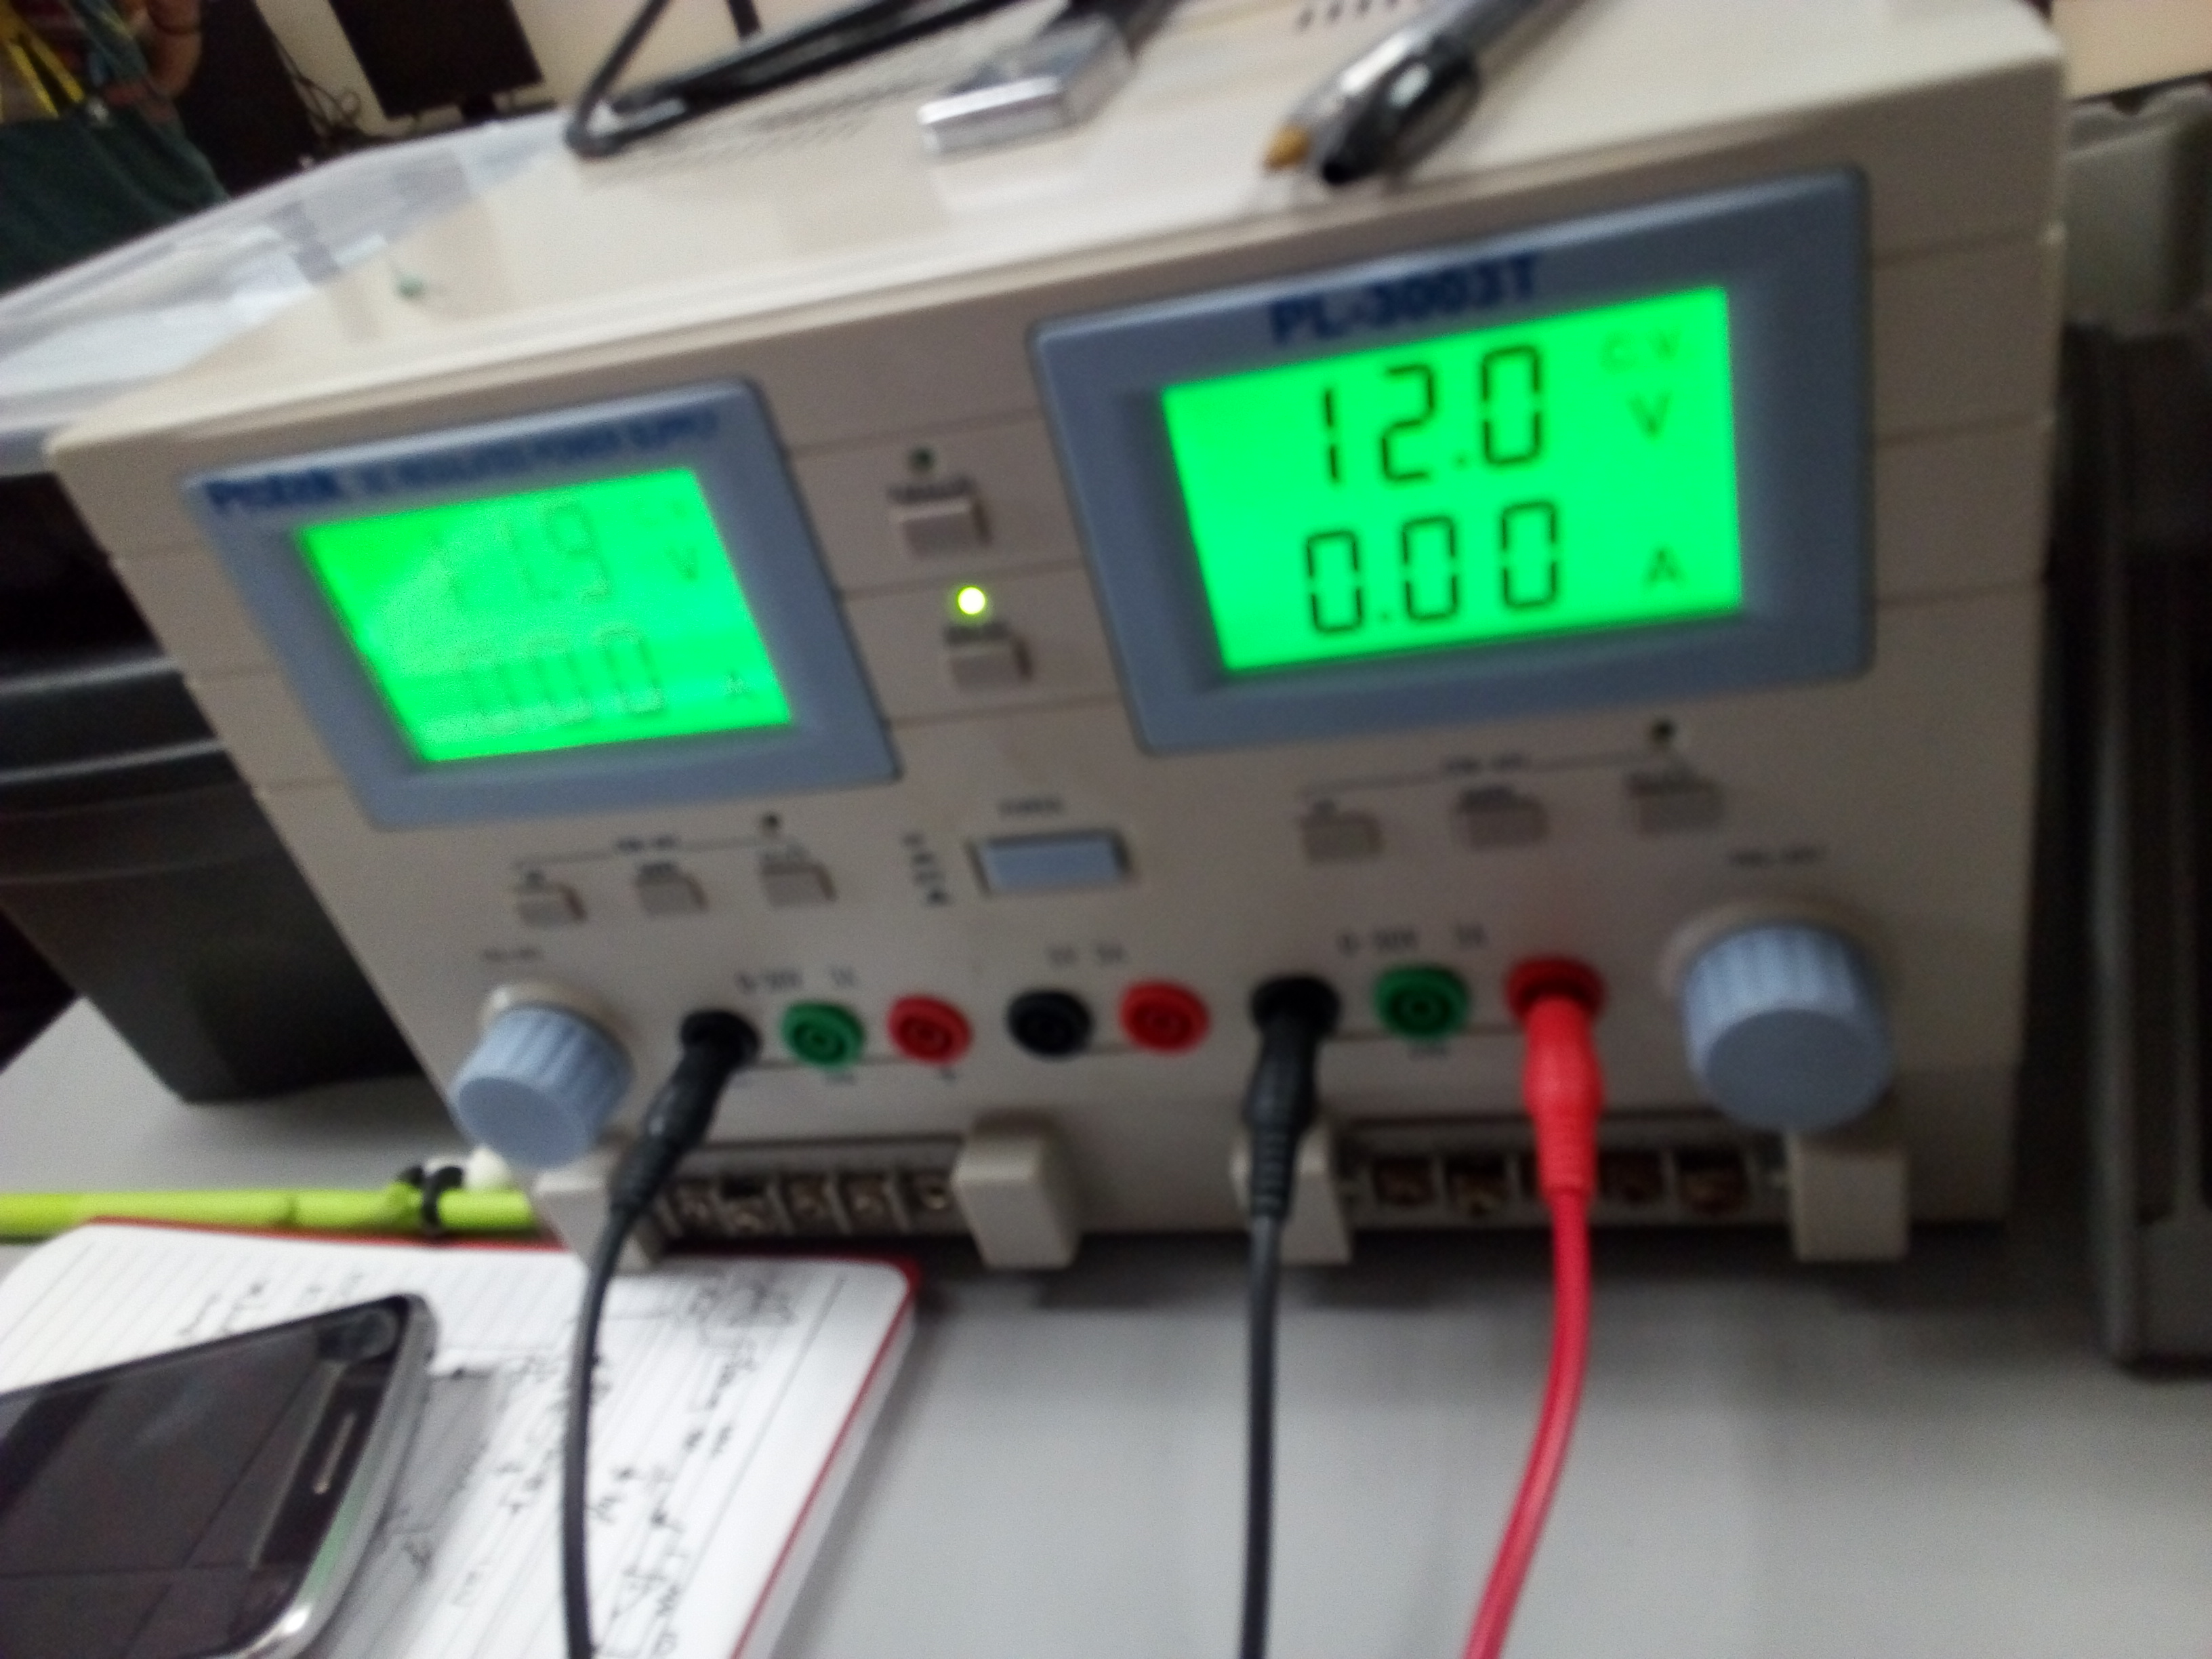
\includegraphics[width=0.7\textwidth]{Sismografo/Images/fuente.jpg}
            \end{figure} 
	       
	    %/////////////////////////////////////////////////////////////////
    	%          CALCULOS PROCEDIMIENTO EXPERIMENTAL 2
    	%/////////////////////////////////////////////////////////////////	    
	    \subsection{PE- 2 Filtrado de señal}
            \begin{enumerate}
        		\item Definición de la frecuencia de corte o $f_{c}$ o $w_{c}$, donde: $w_{c}=2 \pi f$.					\\
        				Con $ f=12Hz $ tenemos que:
        				$$ w_{c}=2\pi (12Hz) = 24 \pi Hz = 75.39 Hz $$
        		\item Definición del capacitor 1 ($C_{1}$), eligiendo un valor comprendido entre $100pF$ y $1\mu F$.	\\
        				Con $C_{1}=1\mu F$.
        		\item Calcular el $C_{2}$,  $C_{2}=2C_{1}$.																\\
        				Con $C_{1}=1\mu F$, tenemos que:
        				$$ C_{2}=2C_{1} = 2(1\mu F) = 2 \mu F $$
        		\item Calcular el resistor R, donde:																	\\
        				$$ R = \frac{0.707}{w_{c}C_{1}} = \frac{0.707}{(75.39 Hz)(1 \mu F)} = \frac{0.707}{75.39\mu} = 9.37 K\Omega $$

        	    \item Finalmente, calcular la resistencia de referencia $R_{Ref}=2R$.\\
        	    Con $R=9.37 K\Omega $, tenemos que:
        	    $$ R_{Ref}=2R = 2(9.37 K\Omega) = 18.75 K\Omega $$
        	\end{enumerate}
        	
	    %/////////////////////////////////////////////////////////////////
    	%          CALCULOS PROCEDIMIENTO EXPERIMENTAL 3
    	%/////////////////////////////////////////////////////////////////	    
		\subsection{PE- 3 Segunda etapa de amplificación}
		
		\begin{enumerate}
        		\item Definimos la ganancia de voltaje $A_{CL}$ en la segunda etapa amplificadora, donde el voltaje pico-pico de entrada es de $V_{i}=880 mV$ y el voltaje pico-pico de salida deseado sera de $V_{o}=10.26 V$
        		
        		Aplicando las fórmulas del Amplificador No Inversor tenemos:

        				$$ A_{CL} = \frac{V_{o}}{V{i}} = \frac{10.26 V}{0.88 V} = 11.66 $$
        				
        				
        	\item Ahora, utilizamos otra formula que igualaremos con la ecuación anterior:
        	
        	$$ A_{CL} =
        				11.66 = 1 + \frac{R_{f}}{R_{i}} $$
        				
            \item Comenzamos a operar en ella. Pasamos el uno restando al otro lado de la igualdad:
            
            $$ 10.66 = \frac{R_{f}}{R_{i}} $$
        	
        	\item Como vemos, obtuvimos una única ecuación pero con 2 incógnitas. Matemáticamente es imposible solucionar esto. Para evitar quedarnos estancados proponemos un valor para cualquiera de las resistencias. En esta caso elegimos $R_{i} = 1.5K\Omega$
        	\\
        	$$ 10.66 = \frac{R_{f}}{1.5K\Omega} $$
            
            \item Pasando multiplicando, obtenemos $R_{f}$
            \\
            $$ R_{f} = (10.66)(1.5K\Omega) = 16K\Omega $$
            
            \item Los valores de las resistencias son: $R_{i} = 1.5K\Omega$ y $R_{f} = 16K\Omega$
        	
        \end{enumerate}
		
		%/////////////////////////////////////////////////////////////////
    	%          CALCULOS PROCEDIMIENTO EXPERIMENTAL 4
    	%/////////////////////////////////////////////////////////////////	    
		\subsection{PE- 4 Vúmetro de led's}
		
		Para justificar nuestra repuesta en el Procedimiento establecido, calculamos el rango con un divisor de Voltaje, como a continuación se muestra:
		
		\begin{enumerate}
		    \item Calculamos el voltaje de salida, y como las resistencias son iguales entonces aplicamos la siguiente ecuación:\\
		    Primero calculamos la Intensidad de corriente para:
		     $$
		        I = \frac{V}{R} = \frac{5V}{9(2.2k\Omega)} = \frac{5V}{19.8k\Omega} = 0.252 mA 
		     $$
		     Recordemos que el voltaje de la fuente de alimentación que va hacia las resistencias de las entradas inversoras de los amplificadores operacionales paso por un regulador de voltaje 7805 y ahora esta a 5V estables.
		     
		     Como es un circuito en serie, la corriente es la misma en todos por lo tanto al sacar el voltaje en cada uno de los operadores tenemos;
		   
		    \begin{equation*}
		        \begin{split}

		             V_{1} &= (R)I = RI = (2.2k\Omega)(0.252mA) = 0.55 V   \\
		            V_{2} &= (R+R)I = (2R)I = (4.4k\Omega)(0.252mA)) = 1.11 V     \\
		            V_{3} &= (R+R+R)I = (3R)I = (6.6k\Omega)(0.252mA) = 1.66 V     \\
		            V_{4} &= (R+R+R+R)I = (4R)I = (8.8k\Omega)(0.252mA) = 2.22 V     \\
		            V_{5} &= (R+R+R+R+R)I = (5R)I = (11k\Omega)(0.252mA) = 2.77 V     \\
		            V_{6} &= (R+R+R+R+R+R)I = (6R)I = (13.2k\Omega)(0.252mA) = 3.33 V     \\
		            V_{7} &= (7R)I = (15.4k\Omega)(0.252mA) = 3.88 V     \\
		            V_{8} &= (8R)I =  (17.6k\Omega)(0.252mA) = 4.44 V     \\

		        \end{split}
		    \end{equation*}
		    
		    Con estos cálculos, justificamos la respuesta de que el rango es de $0.55 V$ a $4.44 V$
		    
		\end{enumerate}

    %/////////////////////////////////////////////////////////////////
	%                           REFERENCIAS
	%/////////////////////////////////////////////////////////////////

	\nocite{ref1, ref2, ref3, ref4}
	\bibliography{referencias}
\end{document}